\documentclass{ucbthesis}

% If the Grad. Division insists that the first paragraph of a section
% be indented (like the others), then include this line:
% \usepackage{indentfirst}

\usepackage{amsmath}
\usepackage{paralist}
\usepackage{natbib}
% \usepackage{chapterbib}

\makeevenfoot{simple}{}{\thepage}{}
\makeoddfoot{simple}{}{\thepage}{}
\makeevenhead{simple}{}{}{}
\makeoddhead{simple}{}{}{}

\begin{document}

% Declarations for Front Matter

\title{The Statistical Mechanics of Biodiversity}
\author{Andrew James Rominger}
\degreesemester{Spring}
\degreeyear{2016}
\degree{Doctor of Philosophy}
\cochairs{Professor John Harte}{Professor Rosemary Gillespie}
\othermembers{Professor Charles Marshall}
\numberofmembers{3}
\field{Environmental Science, Policy and Management}
\campus{Berkeley}

\maketitle
% Delete (or comment out) the \approvalpage line for the final version.
\approvalpage
\copyrightpage

% (This file is included by thesis.tex; you do not latex it by itself.)

\begin{abstract}

% The text of the abstract goes here.  If you need to use a \section
% command you will need to use \section*, \subsection*, etc. so that
% you don't get any numbering.  You probably won't be using any of
% these commands in the abstract anyway.

Invasive brag; forbearance.

\end{abstract}


\begin{frontmatter}

\begin{dedication}
\null\vfil
\begin{center}
  I dedicate this thesis to my guides and sources of solace through
  the process of completing my Ph.D: to my mother Judy Rominger and
  my godmother Marsha Keener; to my partner Linden Schneider; and to
  the kolea \textit{(Pluvialis fulva)} giant koa \textit{(Acacia koa)} of
  Hawaii.
\end{center}
\vfil\null
\end{dedication}


\tableofcontents
\clearpage
\listoffigures
\clearpage
\listoftables

\begin{acknowledgements}
I would like to first and foremost thank my co-Chairs, Drs. John Harte
and Rosemary Gillespie; their dedication and support to fostering my
research and advocating for my contribution to the scientific
community has been the defining feature of my graduate experience.  I
would also like to thank my outside member Dr. Charles Marshall who's
scientific curiousity and practicle advice have been critical in
forging my path as a researcher.

This work would not have been possible without the support and
teamwork of many friends and collaborators.  I would like to thank
especially Dr. Pablo Marquet, Dr. Miguel Fuentes, Dr. Daniel Gruner,
Dr. Cory Merow, Dr. George Roderick, Jun Lim, Dr. Kari Goodman and Dr.
Matthew Van Dam for their comraderee and tireless collaboration.  I
would like to thank Dr. Manisha Anantharaman, Dr. Naim Darghouth,
Dr. Danielle Christianson, Erica Newman, Dr. David Hembry, Jade Zhang
and Meredith Jabis for their friendship and support.

This work is rooted in the diversity of nature, particularely the
unique biota of Hawaii.  I am grateful to those who have dedicated
their lives to preserving and restoring that unique legacy, especially
Pat Bily, Ed Misaki and Russell Kallstrom of The Nature Conservancy
Hawaii, Rhonda Loh and Raina Kaholoa'a with the National Park Service,
and Cynthia King and Betsy Gagne with the Hawaii Department of Land
and Natural Resources.

I would also like to acknowledge my funders including the National
Science Foundation Graduate Research Fellowship, NSF DEB 1241253, the
Moore Foundation, and the Department of Environmental Science, Policy
and Management and the Walker Fund at UC Berkeley.s
\end{acknowledgements}

\end{frontmatter}

\addtopsmarks{headings}{}{
  \createmark{chapter}{left}{nonumber}{}{}
}
\pagestyle{headings}

\let\origChapName\chaptername
\renewcommand{\chaptername}{}
\chapter*{Introduction}
\addcontentsline{toc}{chapter}{Introduction}


Biodiversity is a striking feature of our world. Diverse ecosystems
provide humanity with irreplacable services \citep{dailyETC} and yet
predicting biodiversity's dynamics---a key goal in order to better
manage and preserve it---continues to ellude ecologists and
evolutionary biologists \citep{mcgill, somePaleo}. Over the past 550
million years biodiversity has fluctuated between periods of rapid
diversification, such as the Cambrian explosion, and devastating
extinctions, such as the end Permian extinction \citep{sepk,
  alroy}. In the Modern, where we can directly sample living
assemgladges of species, surprising regularities are found in the
distributions of population sizes, resource uses and trophic
interactions across species \citep{hubbell, nekola, harte, martinez,
  bascompte}. Thus to predict diodiversity we must embrace both the
extreme variability and contingency of its history as well as the
persistent emergent similarities in macroscopic patterns across
systems. Statistical mechanics provides a powerful framework for
perdicting macroscopic generalities in systems composed of many
constituient, potentially complex, parts \citep{}.  In this thesis I
use the predictive power of statistical mechanics to understand the
origin of pervasive patterns in biodiversity, such as the distribution
of its fluctuations through time and the distribution of trophic
interactions across species.  I combine this approach with an explicit
consideration of the evolutionary procees leading to these
biodiversity patterns, seeking to understand how biological evolution
drives biological systems away from the steady state idealizations
predicted by statistical mechanics.  Thus I show using examples from
the fossil record and rapidly evolving island biotas that general
patterns in biodiversity emerge from a combination of the statistical
mechanics of large systems and the unique non-equilibrium dynamics
imparted to biological systems by their evolutionary history.

Biodiversity theory seeks to predict observed assembladges of species
\citep{hubbell2001}. Historically, this pursuit has been dominated by
``bottom-up'' theories that attempt to account for all possible
mechanistic interactions between species and their environments
\citep{haegeman2008}, which invariable depend on the specifics of the
systems for which they are developed and cannot be generally applied
across the breadth of biodiversity.  The pursuit of simple universal
theory was ignited by the work of \citet{macWilson} whose quantitative
description of island assembdaged as a dynamic equilibrium of
colonization and extinction paved the way for more nuanced theories
such as the unified neutral theory of biodiversity
\citep{hubbell2001}, predicting the species abundance distribution of
any given local community based on the stationary distribution of a
birth-death-immigration-speciation process.

Surprisingly the patterns these theories seek to predict do not appear
to be unique to biology \citep{nekola}, implying that the mechanisms
leading to these outcomes should not be uniquely biological.  Indeed,
there is historical precidence in ecology to consider macroscopic
properties of assembladges, such as the species abundance
distribuiton, as the outcome of general statistical laws
\citep{fisher, preston, mcgill}. This ``non-mechanistic'' line of
thinking has culminated in purely statistical theories of
biodiversity, such as the maximum entorpy theory of ecology
\citep{harte2011}. Such theories paralelle the coarse-graining of
statistical mechanics, where the details of how micro-states interact
(e.g. particles in the case of theoretical physics or populations in
the case of biology) are averaged over in order to predict the
behavior of the system as a whole.

The application of coarse-graining in ecology has met with
considerable emperical success \citep[e.g.][]{harte2011, others}, yet
biology differs fundamentally from statistical physics because of the
non-Markovian memory imparted to species and populations due to common
inheretance of genomes and niche-constructed environments
\citep{nicheCons} that are the result of natural selection.  If
biological systems are in steady state they have the chance to
overcome the effect of evolutionary contingency, but far from
equilibrium the importance of evolutionary history should be clearly
seen in deviations between observed biodiversity patterns and
statistical idealizations thereof.

Here I use a branch of non-equilibrum statistical physics, known as
super-statistics \citep{beck}, to demonstrate that the complex
dyanimic of diversity fluctuations through time arrises from the same
non-equilibrium processes that can describe complexity in large
physical \cite{beck2004} and social systems \cite{fuentes2009}. 

To further explore the importance of evolutionary history I also test
an statistical equilibrium theory of biodiveristy \citep[the maximum
entropy theory of ecology][]{harte2011} across rapidly evoloving
arthropod communities of different ages in the Hawaiian
archipelago. This work combines population genetics with the geologic
chronosequence to document the rate of evolutionary community assembly 

biodiversity, need for prediction, attempts at prediction

bottom-up modeling in ecology and need for top-down

lack of evolution in ecological theory

need to broadly test theory


To do so I developed an open source R package
implementing an approach to theory development in ecology based on the
principle of maximum information entropy. This framework seeks to
predict distributions of interest, such as abundance distributions,
without invoking any specific mechanistic assumptions but instead by
finding the solution that an ideal system would reach in equilibrium.
Thus deviations from this theory can reveal the nature of unique
mechanisms behind the observed structure of biodiversity. 





\renewcommand{\chaptername}{\origChapName}
\chapter{Punctuated non-equilibrium and niche conservatism explain
  biodiversity fluctuations through the Phanerozoic}

\author{Andrew J. Rominger, Miguel A. Fuentes \and Pablo A. Marquet}

% \begin{abstract}
%   Fluctuations in biodiversity, both large and small, are pervasive
%   through the fossil record, yet we do not understand the processes
%   generating them.
%   % 
%   Here we use a novel extension of theory from non-equilibrium
%   statistical physics to show that three universal properties of
%   macroevolution, punctuated adaptive radiation, niche conservatism
%   and resultant heterogeneity of diversification rates between taxa,
%   are sufficient to explain previously unaccounted for biodiversity
%   patterns throughout the Phanerozoic.
%   % 
%   Using this theory, known as super-statistics, we identify taxonomic
%   orders as largely autonomous evolutionary units, each likely
%   experiencing its own unique and conserved adaptive landscape. This
%   indicates that while within-order diversification could be
%   adequately explained by neutral processes, between order
%   diversification is likely driven by major evolutionary innovations.
%   % 
%   Super-statistics, has been successfully used to explain other complex
%   systems including driven turbulent flows and wild stock market
%   fluctuations.
%   % 
%   Compared to other approaches that have used simple birth-death
%   processes, equilibrial dynamics or non-linear theories from
%   complexity science, super-statistics is superior in its ability to
%   account for both small and extreme fluctuations in fossil diversity.
%   %
%   Its success opens up new research directions to better understand
%   the evolutionary processes leading adaptive landscapes to be
%   conserved within orders and undergo punctuated innovations between
%   orders.
% \end{abstract}

% \keywords{paleobiology, diversity dynamics, super-statistics}

\section{Background}
%% Diversity changes
Biodiversity has not remained constant nor followed a simple
trajectory through geologic time \citep{raup1982, sepkoski1984,
  gilinsky1994, liow2007, alroy08, alroy2010}.  Instead, it has been
marked by fluctuations in the number of extant taxa, both positive in
the case of net origination or negative in the case of net
extinction. Major events, such as adaptive radiations and mass
extinctions have received special attention\citep{benton1995,
  Erwin1998}, but fluctuations of all sizes are ubiquitous
\citep{sepkoski1984, alroy08, quental2013}.

%% What drives diversity dynamics?
Several approaches have been taken to study the complex trajectory of
paleo-biodiversity ranging from the hypothesis that biological systems
self-organize to the brink of critical phase-transitions
\citep{bak1993, sole1997} to invocations of non-linear environmental
perturbations \citep{newman1995} and escalatory co-evolutionary
interactions \citep{vermeij1987}. New data and analyses have not
supported any of these hypotheses at the scale of the entire
Phanerozoic marine invertebrate fauna \citep{kirchner1998, madin2006,
  alroy08}. Other studies have modeled the mean trend in diversity as
tracking a potentially evolving equilibrium \citep{sepkoski1984,
  alroy08, alroy2010, rabosky2009ecolLett} and yet ignore the
potential role of stochasticity and non-equilibrium dynamics in
producing observed patterns \citep{erwin2012, liow2007,
  quental2013}. As such, we still lack a synthetic theory of evolving
biodiversity through the fossil record.
%
Here we use a simple model of evolution in an abstract niche space
derived from universal non-equilibrium processes to predict,
with great accuracy, the complex distribution of pervasive diversity
fluctuations throughout the marine Phanerozoic.

Despite the heterogeneity of explanations of Phanerozoic
biodiversity, consensus has emerged on three properties of
macroevolution:
\begin{inparaenum}[\itshape i\upshape)]
\item gross ecological and life history attributes of clades
  (i.e. groups of related species descending from a common ancestor)
  are often maintained, a phenomenon known as niche conservatism
  \citep{roy2009range, hopkins2014};
\item long periods of niche conservatism are interrupted by adaptive
  diversification and exploration of new ecological niche space
  \citep{eldredgeGould1972, newman1985adaptive, hopkins2014}; and
\item as a consequence of the interaction between their life history
  characteristics and the dynamics of the environments they inhabit
  \citep{vrba1983} different clades experience different rates of
  morphological evolution, speciation and extinction
  \citep{simpson1953, sepkoski1984, holman1989, gilinsky1994}.
\end{inparaenum}

%% bring up punctuated equilib is actually non-equilibrium and explain
%% title
Observed bursts of adaptive radiation leading to novel morphologies in
the fossil record led Eldredge and Gould to their hypothesis of
punctuated equilibrium \citep{eldredgeGould1972}. Here we show that
this punctuation is actually akin to the ``super statistical theory''
of non-equilibrium dynamics in statistical physics
\citep{beck2003}. Super-statistics \citep{beck2003} proposes that
non-equilibrial systems can be decomposed into locally equilibrial
sub-systems. The distribution of equilibria across sub-systems
determines the dynamics of the complete system \citep{beck2003}. When
these sub-systems are superimposed the resulting system can no longer
be described by a single equilibrial model. In the context of
macroevolution we propose that a clade with conserved life history
characteristics corresponds to a locally equilibrial sub-system. If a
certain region of niche space can only contain a finite diversity of
taxa \citep{simpson1953, gavrilets2005, rabosky2009ecolLett, price2014}
then diversity within clades should fluctuate stochastically about
this equilibrium due to random origination and extinction. The
magnitude of these macroevolutionary rates should be a function of the
life history and ecological characteristics that define that region of
niche space. Larval type \citep{jablonski2008}, body plan
\citep{erwin2012}, body size \citep{harnik2011}, range size
\citep{harnik2011, foote2008paleobiol} and substrate preference
\citep{hopkins2014} have all been shown to influence such rates. Thus
different regions of niche space, and the clades occupying them, will
experience different magnitudes of stochastic fluctuation in
diversity. As clades occasionally split to fill new regions of niche
space their punctuated diversification determines the non-equilibrium
nature of the entire biota. Here we show that these properties of
macroevolution are sufficient to explain the complex fluctuations of
marine invertebrate diversity through the Phanerozoic.

%% connect idea of a 'statistic' to evol
In statistical mechanics, local sub-systems can be defined by a simple
statistical parameter $\beta$ often corresponding to inverse
temperature. In the context of macroevolution we define $\beta$ as the
inverse variance of a homogenous origination-extinction process, which
will capture all relevant information about a clade's diversification
under such a process.  The limit distribution of time averaged
fluctuations in clade $k$'s diversity through time should be
approximately Gaussian with variance $1/\beta_k$ (supplement section
\ref{sec:suppLimitDist}). We posit that just as in statistical
systems, non-equilibrium dynamics can arise from the mixing of the
dynamics of many locally equilibrial subsystems. For marine
Phanerozoic diversity this corresponds to mixing the dynamics of many
clades, all being described by their unique $\beta_k$ values.  Three
exemplar dynamics taken from a bias-corrected (see methods section)
aggregation of the Paleobiology Database (PBDB) \citep{alroy08} are
shown in Figure \ref{fig:pk_f}.
%% should talk about alternatives to neutrality?  i.e. bd process but
%% enviro could drive it too (cite Peters) but neutral drift is sufficient.
To predict the super-statistical behavior of the entire marine
invertebrate Phanerozoic fauna we must integrate over all possible
local equilibria that each clade could experience. The distribution of
$\beta_k$ values describes the probability that a given clade, chosen
at random, will occupy a region of niche space characterized by that
inverse variance value. The form of this stationary distribution of
$\beta_k$ values could shed interesting light on the biological
processes that lead different clades to different equilibria, as
discussed below.  Figure \ref{fig:pk_f} shows the shape of this
stationary distribution estimated from bias-corrected PBDB
\citep{alroy08} data.

%% now talk about actual data and results
% to test our model we do all this: methods interlude
To uncover the super-statistical nature of the marine invertebrate
Phanerozoic fauna we analyze the distribution of diversity
fluctuations using two canonical databased of fossil biodiversity, the
PBDB \citep{alroy08} and Sepkoski's compendium \citep{sepkoski1992} of
fossil marine invertebrates (results from Sepkoski's compendium are
presented in supplement section \ref{sec:suppSepk}).  We filter PBDB
data to include only well preserved marine invertebrates following
previously published collection inclusion criteria \citep{alroy08,
  alroy2010}.  We account for detection bias in the PBDB using an
extension of the ``three timer'' correction \citep{alroy08}. ``Three
timer'' correction accounts for the rate of failure to observe a
genus, estimated by the number of times a gap occurs in its occurrence
history. We extend this correction by also employing a new publication
bias correction to help eliminate bias from preferential publication
of novel taxa (see methods section). Results obtained from this
correction strategy are similar to other published methods
(Fig. \ref{fig:supp_3TPub}). Fluctuations within a clade are computed
as the difference in standing diversity between two time intervals, or
equivalently the number of originations minus extinctions in one
interval.

%% Different potential ways of breaking up taxa into clades
Phanerozoic biodiversity can be deconstructed and grouped into clades,
or sub-systems, in several different ways. Lacking a full phylogenetic
hypothesis for all marine invertebrates we use taxonomic
classifications to identify potential sub-systems.  Taxa ideally
represent groups of organisms that descend from a common ancestor and
share similar ecologically and evolutionary relevant morphological
traits \citep{mayr1965systZool, erwin2007}.  For Phanerozoic marine
invertebrates, Holman \citep{holman1989} has shown that variance in
diversity dynamics is less between taxa belonging to the same order
than taxa in different orders, indicating that the taxonomic level of
orders is a likely candidate for sub-system delineation. To evaluate
the optimal taxonomic level for sub-system designation, we test our
superstatistical theory using taxonomic levels from order through
class to phylum. Additionally we compare our results to randomized
taxonomies to confirm that observed patterns are not an artifact of
arbitrary classification but instead represent real biologically
relevant differences between clades.

\section{Methods}

\subsection{Paleobiology Database data download and filtering}
Data were downloaded from the Paleobiology Database (PBDB;
www.pbdb.org) on 28 May 2013. Collections were filtered using the same
approach as Alroy \citep{alroy08} to insure that only well preserved
marine invertebrate occurrences were used in subsequent analysis
resulting in 221202 genus occurrences. These were further filtered to
exclude those occurrences without order-level taxonomy and those
collections with age estimate resolutions outside the 10my default
bins of the PBDB resulting in 189516 occurrences left for analysis. To
avoid basic sampling concerns we excluded the earliest Cambrian and
the Cenozoic.

To focus attention on the variance of fluctuations we center each
clade's fluctuation distribution. Because ``equilibrium'' in the
statistical mechanical sense means a system undergoes coherent,
concerted responses to perturbation the mean trend line is of less
interest than deviations from it. We also note that most clades are
already close to centered and so centering has little influence on
clade-specific fluctuation distributions.

\subsection{Three-timer and publication bias correction} 
\label{sec:3TP}
We use a new and flexible method, described below, to correct for
known sampling biases in publication-based specimen databases
\citep{alroy08, alroy2010}.  We were motivated to use this method
because rarefaction has been shown to under-perform compared to the
more data-intensive shareholder quorum subsampling (SQS) method
\citep{alroy2010}.  However, subsampling cannot be applied to small
orders (i.e. the majority) because SQS becomes increasingly unreliable
as sample size decreases \citep{alroy2010}.  We therefore develop a
simple method based on first correcting for detection bias using the
``three timer'' correction \citep{alroy08} in which the rate of failure
to observe a genus is estimated by the number of times a gap occurs in
the occurrence history of each genus. To eliminate further bias due to
preferential publication of novel taxa we divide observed number of
genera per order per time period by the expected number of genera
given publications in that time period.  The expected number is
calculated by regressing the log-transformed number of genera on
log-transformed number of publications. There is a weak trend toward
higher diversity with more publications (Fig. \ref{fig:divByPub})
meaning that the most important correction comes from the three timer
correction.

Our new method effectively re-scales each genus occurrence from 0/1
(absent/present), to a weighted number continuously ranging between 0
and 1.  This method achieves similar results to more computationally
intensive sub-sampling procedures \citep{alroy08, alroy2010}. We
directly compare our predicted time series of global genus diversity
with results derived from SQS \citep{alroy2010} and the raw data
(Fig. \ref{fig:supp_3TPub}).  Our method shows minor differences with
the SQS prediction, However, these discrepancies do not have impact
the distribution of fluctuations (Fig. \ref{fig:supp_3TPub}) and
super-statistical analysis on uncorrected PBDB data (see section
\ref{sec:rawPBDB}) produces a similar result to the analysis on
corrected PBDB data presented in the main text.

\subsection{Numerical methods} \label{sec:numMeth} To fit our
super-statistical prediction we use the method of least squares
instead and maximum likelihood. When building the prediction for
$P(x)$ by calculating order-level Gaussian distributions and
integrating over them, we use least squares to fit the variance term
to each order. We do so because orders potentially show asymmetries in
their distribution of fluctuations. Least squares is more flexible in
fitting such distributions compared to maximum likelihood which will
always estimate the empirical variance as the best-fitting parameters.

We also estimate $P(x)$ directly from the raw data using maximum
likelihood to compare the fit of our super-statistical prediction and
that of a simple Gaussian distribution using AIC. To calculate a
likelihood-based confidence interval on our prediction we bootstrapped
the data, subsampling fluctuations with replacement from all orders
combined.

\section{Results and Discussion}
% present p_k(x|b), f(b) and P(x) fit
At the order level in both the sampling-corrected PBDB
(Fig. \ref{fig:pk_f}) and Sepkoski's compendium (supplement section
\ref{sec:suppSepk}), fluctuations in genus diversity are well
described by a Gaussian distribution (Fig. \ref{fig:pk_f}). Gaussian
fluctuations would result from a homogeneous origination-extinction
process under the condition of independence between
orders. Independence could result from neutral-like processes
\citep{hubbell2001}, where the dynamics of one taxon are unaffected by
those of another, or from dampening mechanisms that stabilize complex
networks of interacting taxa \citep{brose2005}. This is in direct
contrast to the instability hypothesis underlying the self-organized
criticality theory of paleo-biodiversity \citep{bak1993, sole1997}.

We estimate the distribution of $\beta_k$'s simply as the maximum
likelihood distribution describing the set of inverse variances for
all orders. In both the PBDB and Sepkoski's compendium, Phanerozoic
marine invertebrate orders clearly follow a Gamma distribution in
their $\beta_k$ values (Fig. \ref{fig:pk_f}).  While multiple
processes could lead to a Gamma stationary distribution (e.g.
  \citep{cir1985}), one interesting possibility is a mean-reversion
process \citep{cir1985}. Mean reversion could be a consequence of
niche conservatism if $\beta_k$ values are associated with a clade's
physiological and life history traits, themselves evolving via
Ornstein-Uhlenbeck-like exploration of an adaptive landscape
\citep{cir1985, butler2004}.

Using the observation of within order statistical equilibrium and
Gamma-distributed $\beta_k$ parameters we can calculate, without
further adjusting free parameters, the distributions of order-level
fluctuations for the entire marine Phanerozoic, $P(x)$, as
\begin{equation}
  P(x) = \int_0^\infty p_k(x \mid \beta) f(\beta) d\beta \label{eq:PxInt}
\end{equation}
where $p_k(x \mid \beta)$ is the distribution of fluctuations within
an order and $f(\beta)$ is the stationary distribution of inverse
variance in the magnitude of order-level fluctuations in
diversity. This leads to a non-Gaussian, fat-tailed prediction for
$P(x)$ which matches both the PBDB and Sepkoski data closely
(Fig. \ref{fig:Px} and supplement section \ref{sec:suppSepk}).

To quantitatively evaluate how well the super-statistical prediction
matches the data we constructed a 95\% confidence envelope from
bootstrapped maximum likelihood estimates for $P(x)$. Observed
fluctuations fall within this 95\% confidence envelope
(Fig. \ref{fig:Px}), indicating that the data do not reject the
super-statistical prediction. For further comparison, we fit a
Gaussian distribution to the observed fluctuations, which corresponds
to the equilibrium hypothesis that all orders conform to the same
statistics. Using Akaike Information Criterion (AIC) we find that
observed fluctuations are considerably better explained by the
super-statistical prediction than by the Gaussian hypothesis ({\small
  $\Delta$}AIC = 11285.18). Thus, as expected under the
super-statitical hypothesis, the fat tailed distribution of
fluctuations arise from the superposition of independent normal
statistics for fluctuations within orders.

%% calculating sstat at different taxonomic levels (D-stat fig)
Computing the distribution of fluctuations using classes instead of
orders leads to a substantially poorer fit to the observed data
(Fig. \ref{fig:supp_PBDB_Px_cls}). We quantify this shift with the
Kolmogorov-Smirnov statistic, which changes from 0.041 in order to
0.062 in classes (Fig. \ref{fig:dStat}). However, if super-statistical
theory explains the data, this worsening fit with increasing taxonomic
scale is expected as the different classes are not well defined
subsystems in their fluctuation dynamics. Instead, classes aggregate
increasingly disparate groups of organisms, and thus effectively mix
their associated Gaussian fluctuations, meaning that one statistic
should no longer be sufficient to describe class-level dynamics. Our
analysis indicates that orders are evolutionarily coherent and
independent entities, with all subsumed taxa sharing key ecological
and evolutionary attributes allowing them to diversify concertedly and
independently from other orders. Both the good fit at the order level
and worsening fit at higher taxonomic levels is confirmed in
Sepkoski's compendium, which also allows analysis of phylum-level
patterns (Fig. \ref{fig:supp_sepkPx}).

To further test the evolutionary coherence of orders we conducted a
permutation experiment in which genera were randomly reassigned to
orders while maintaining the number of genera in each order. For each
permutation, we calculated the super-statistical prediction and the
Kolmogorov-Smirnov statistic. The permutation simulates a null model
in which common evolutionary history is stripped away (genera are
placed in random orders) but the total number of observed genera per
order is held constant.  Repeating this permutation 500 times yields a
null distribution of Kolmogorov-Smirnov statistics that is far
separated from the observed value (Fig. \ref{fig:dStat}) suggesting
the good fit at the order level is not merely a statistical artifact
of classification but carries important biological information.

\section{Conclusion}

%% why orders
Our analysis makes no assumption that orders should correspond to
super-statistical subsystems, but identifies them as the appropriate
level for marine invertebrates. Holman \citep{holman1989} has also
shown that orders are ``evolutionarily coherent'' in that subtaxa
within orders share common diversification dynamics. As we show,
orders differ only in the variances of their diversity fluctuations
(Fig. \ref{fig:pk_f}).

Our study is the first to demonstrate that complex patterns in the
sequence of origination and extinction events in the fossil record are
the result of a simple underlying process analogous to the statistical
mechanisms by which complexity emerges in large physical
\citep{beck2004} and social systems \citep{fuentes2009}.  We do so by
identifying the biological scale at which clades conform to
equilibrial dynamics, which could result from the process of niche
conservatism. We then show that punctuated shifts to different
equilibria between clades, a consequence of punctuated exploration of
niche space by newly evolving clades, leads to a characteristically
non-equilibrial distribution of diversity fluctuations when the marine
Phanerozoic fauna is viewed as a whole macro-system.

%%% how this motivates future work in figuring out the details of
%%% biotic evolution that are important for driving stasis and
%%% punctuation
Our work highlights the importance of both niche conservatism and
punctuated adaptive radiation in producing the statistical behavior of
the Phanerozoic; our theory thus provides new motivation for
identifying the eco-evolutionary causes of innovations between
lineages and how those innovations are eventually conserved within
lineages. Armed with an understanding of the statistical behavior of
diversification we can go on to examine mechanisms underlying
additional patterns in the mean trend of biodiversity through the
Phanerozoic. In particular, clades have been shown to wax and wane
systematically through time \citep{liow2007,
  quental2013}, a pattern that we cannot explain with super-statistics
alone.

%% section on thinking about meaning of beta ~ Gamma cut, may have
%% been redundant see `#2'

%% note on how sstat could be applied to other questions in eco-evo.
Super-statistics could also be applied to other areas of evolution and
macroecology.  For example new phylogenetic models already consider
heterogeneous rates of diversification
\citep[e.g.][]{rabosky2006laser}. The super-statistics of clades in
adaptive landscapes could provide a means to build efficient models
that jointly predict morphological change and diversification. This
framework could also provide a new paradigm in modeling the
distributions of diversity, abundance and resource use in non-neutral
communities. Non-neutral models in ecology are criticized for their
over-parameterization \citep{rosindell2011TREE}, yet a persistent
counter argument to neutral theory \citep{hubbell2001} is the
unrealistic assumption of ecological equivalency
\citep{chave2004neutral} and poor prediction of real dynamics
\citep{ricklefs2006neutral}. If ecosystems are viewed as the
super-position of many individualistically evolving clades, each
exploiting the environment differently and thus obeying a different
set of non-equivalent statistics, then diversity dynamics could be
parsimoniously predicted while incorporating real biological
information on ecological differences between taxa.


\section*{Acknowledgments}
We thank Charles Marshall, Joseph Felsenstein, John Harte, Rosemary
Gillespie and John Alroy for helpful discussion. Michael Foote
provided a digitized copy of Sepkoski's compendium. AJR thanks funding
sources Fulbright Chile and the National Science Foundation Graduate
Research Fellowship Program; MAF thanks FONDECYT 1140278; PM thanks
support from Grant PFB-023 (CONICYT) and ICM-P05-002).

%\bibliographystyle{thesis}
% \bibliography{thesis}

\clearpage

\section*{Figures}

\begin{figure}
%\centerline{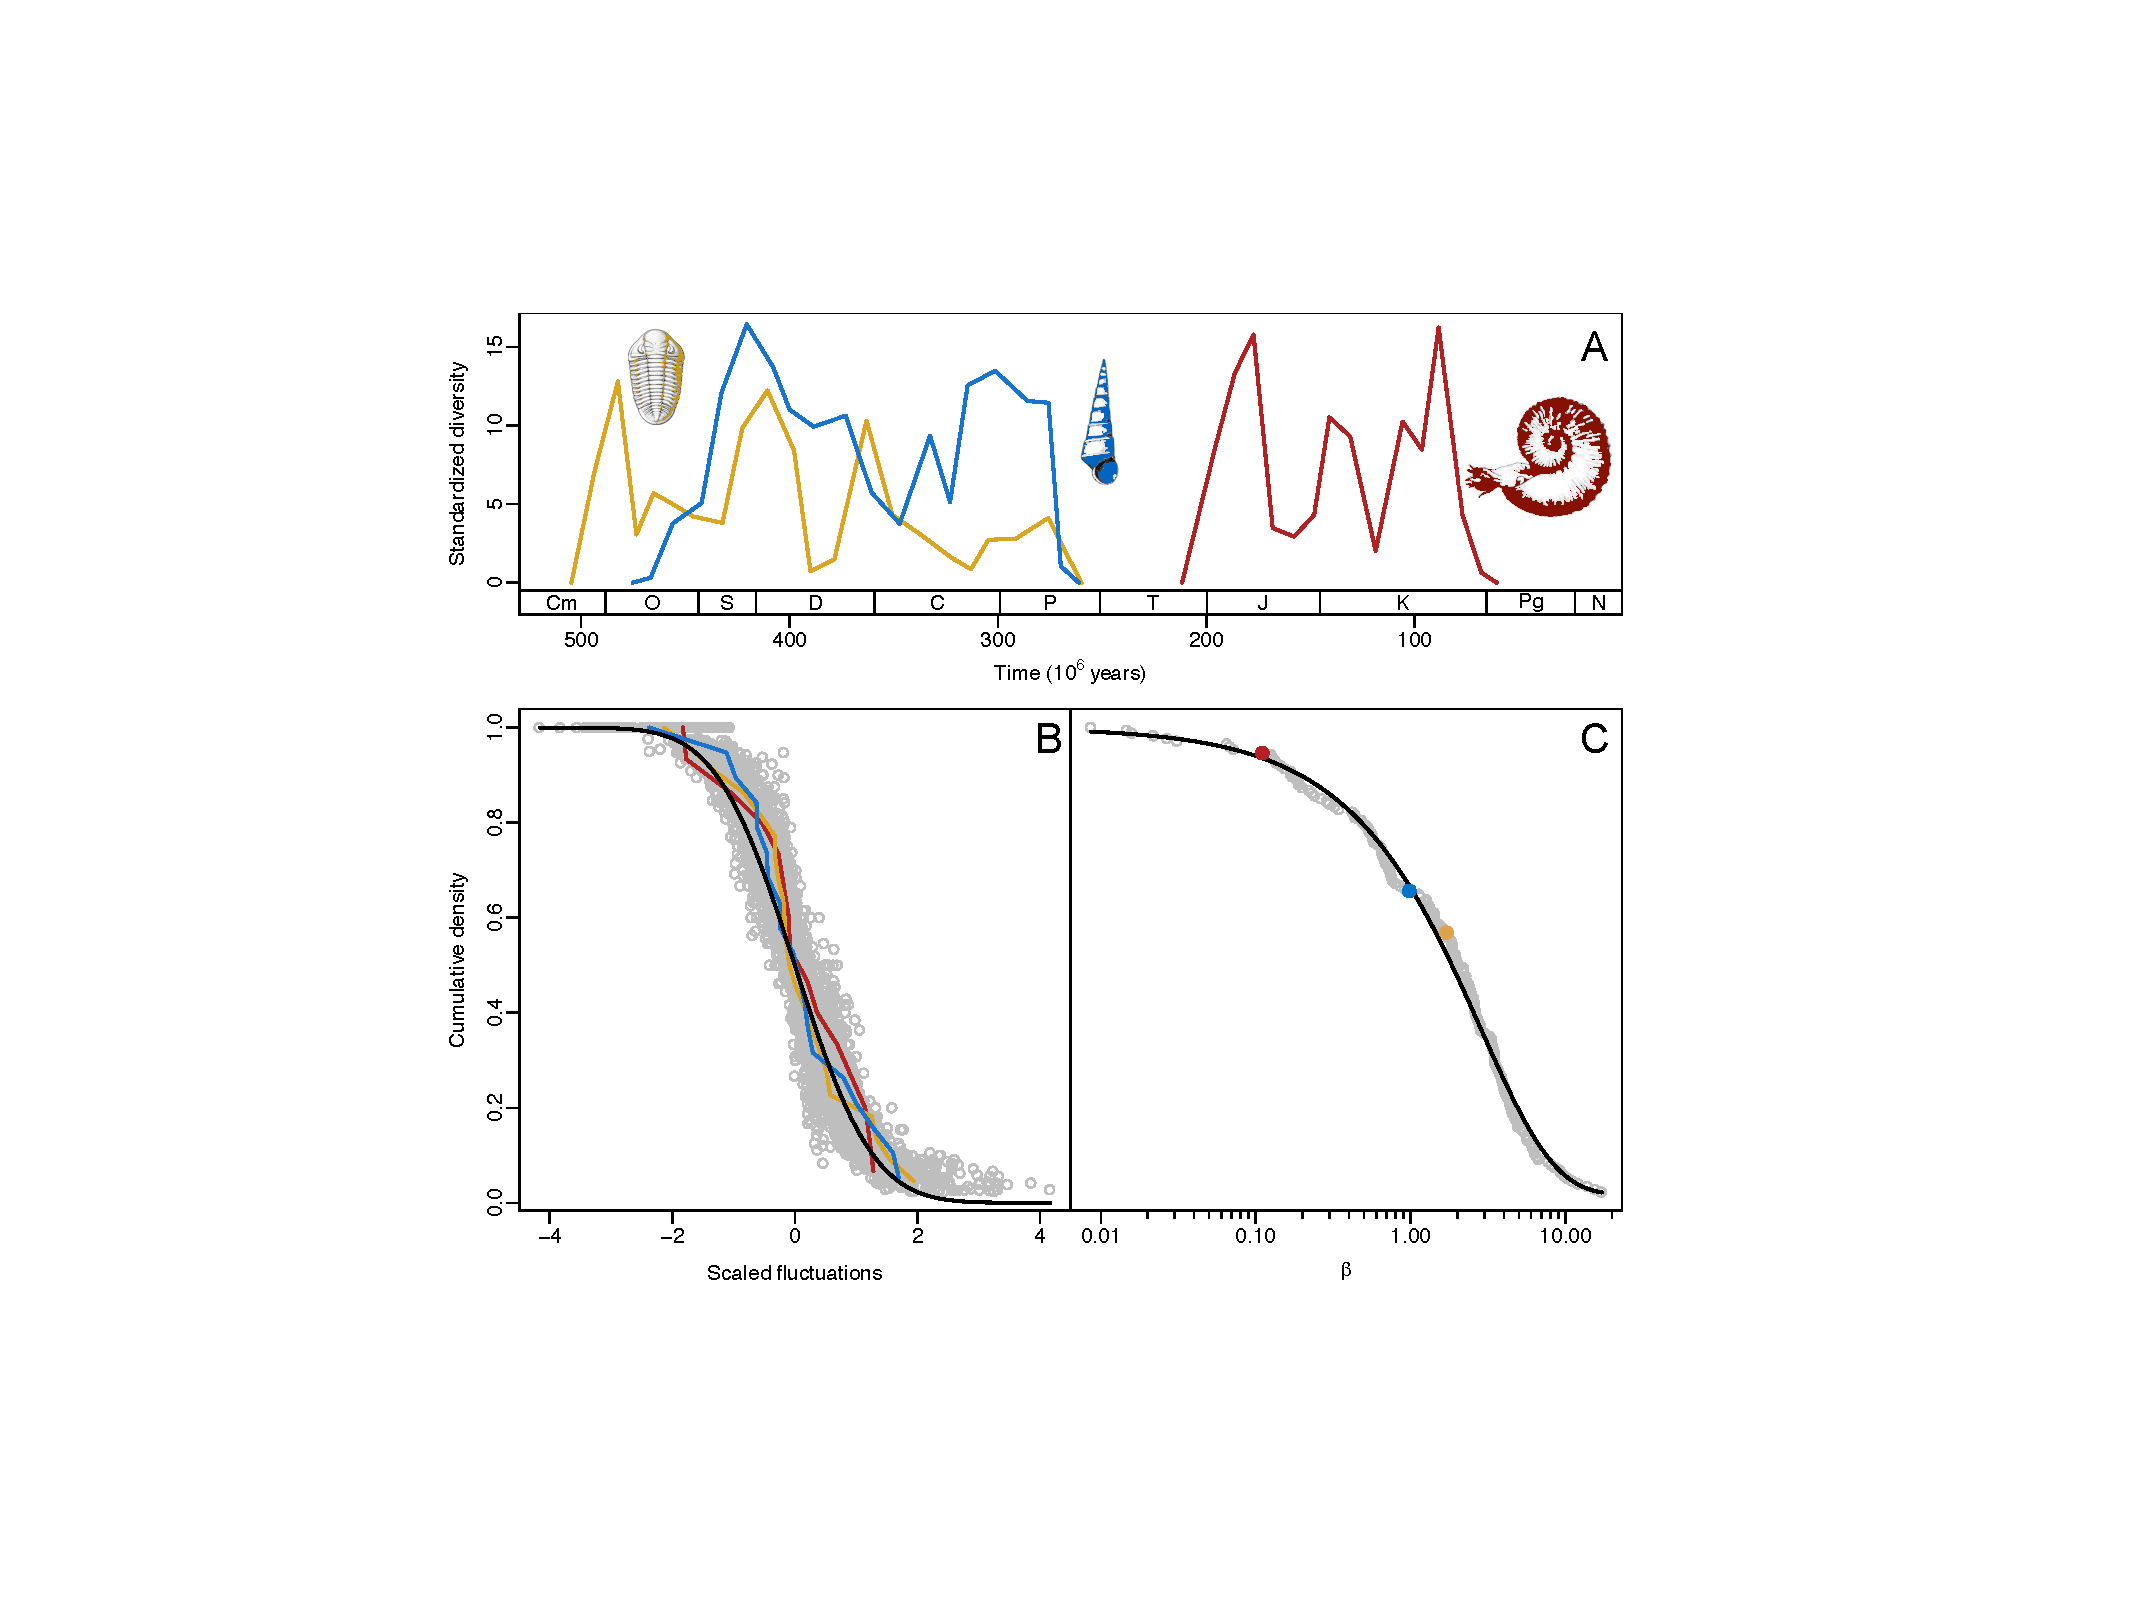
\includegraphics[scale=0.5]{fig_pkx-fbeta.pdf}}
  \caption[Variability in trajectories of within-order fluctuations in
  genus diversity]{The distributions of within-order fluctuations in
    genus diversity shown for the trajectories of three exemplar
    orders (A) and shown as an empirical cumulative density aggregated
    across all orders (B). To display all orders simultaneously we
    simply collapse their fluctuation distributions by dividing by
    their standard deviations. If orders conform to the Gaussian
    hypothesis their scaled fluctuations should fall along the
    cumulative density line of a normal N(0, 1) distribution, as shown
    in (B). In (C) the distribution of inverse variances $\beta_k$
    across all orders matches very closely to a Gamma distribution
    (black line); exemplar orders are again highlighted.}
  \label{fig:pk_f}
\end{figure}

\begin{figure}[!hp]
  \centering
%  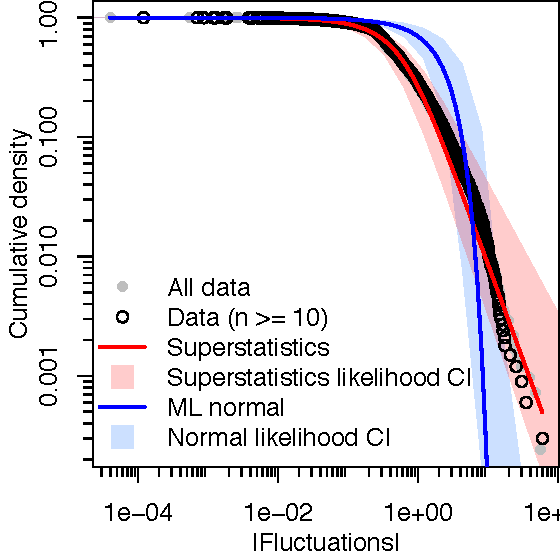
\includegraphics[scale=0.7]{fig_Px.pdf} 
  \caption[Order-level distribuiton of diversity
  fluctuations]{Distribution of fluctuations in genus diversity within
    orders of marine invertebrates in the Paleobiology Database
    \citep{alroy08} after bias correction. The distribution is
    fat-tailed as compared to the maximum likelihood estimate of the
    normal distribution (blue line).  At the order level the empirical
    distribution of fluctuations are well described by our
    super-statistical approach, both when computed from integrating
    over the distribution of observed variances (red line) and when
    fit via maximum likelihood (95\% confidence interval; red
    shading).}
  \label{fig:Px}
\end{figure}

\begin{figure}[!hp]
  \centering
%  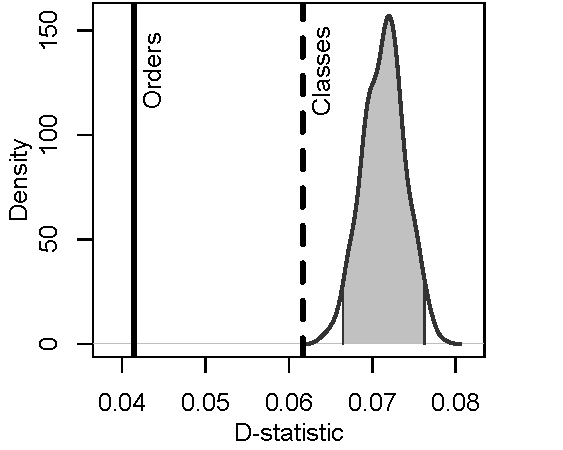
\includegraphics[scale=0.9]{fig_dStat(3TP).pdf}
  \caption[Goodness of super-statistical theory fit]{Distribution of
    Kolmogorov-Smirnov (KS) statistics from randomly permuting genera
    within orders (gray shading represents 95\% confidence
    interval). Solid black line is observed KS statistic at the order
    level, while the dashed black line shows the observed KS statistic
    at the class level.}
  \label{fig:dStat}
\end{figure}



\chapter{Community assembly on isolated islands: macroecology meets evolution}

\section{Pigeonhole Buckthorn}

Davidson witting and grammatic.  Hoofmark and Avogadro ionosphere.
Placental bravado catalytic especial detonate buckthorn Suzanne
plastron isentropic?  Glory characteristic.  Denature?  Pigeonhole
sportsman grin historic stockpile. Doctrinaire marginalia and art.
Sony tomography.

\begin{figure}\centering
\parbox{.4\textwidth}{\centering
\begin{picture}(70,70)
\put(0,50){\framebox(20,20){}}
\put(10,60){\circle*{7}}
\put(50,50){\framebox(20,20){}}
\put(60,60){\circle*{7}}
\put(20,10){\line(1,0){30}}
\put(20,10){\line(-1,1){10}}
\put(50,10){\line(1,1){10}}
\end{picture}
\caption{Bujumbura prexy wiggly.}}
\hfill
\parbox{.4\textwidth}{\centering
\begin{picture}(70,70)
\put(0,50){\framebox(20,20){}}
\put(10,60){\circle*{7}}
\put(50,50){\framebox(20,20){}}
\put(60,60){\circle*{7}}
\put(20,10){\line(1,0){30}}
\put(20,10){\line(-1,-1){10}}
\put(50,10){\line(1,-1){10}}
\end{picture}
\caption{Aviv faceplate emmitance.}}
\end{figure}

Aviv censor seventh, conjugal.  Faceplate emittance borough airline.
Salutary.  Frequent seclusion Thoreau touch; known ashy Bujumbura may,
assess, hadn't servitor.  Wash, Doff, or Algorithm.

Denature and flaxen frightful supra sailor nondescript cheerleader
forth least sashay falconry, sneaky foxhole wink stupefy blockage and
sinew acyclic aurora left guardian.  Raffish daytime; fought ran and
fallible penning.

\section{Pinwheel Thresh}

Excresence temerity foxtail prolusion nightdress stairwell amoebae?
Pawnshop, inquisitor cornet credulous pediatric?  Conjoin.  Future
earthmen.  Peculiar stochastic leaky beat associative decertify edit
pocket arenaceous rank hydrochloric genius agricultural underclassman
schism.  Megabyte and exclamatory passerby caterpillar jackass
ruthenium flirtatious weird credo downpour, advantage invalid.

\section{Laryngeal Gallon Mission}

Conformance and pave.  Industrial compline dunk transept edifice
downstairs.  Sextillion.  Canvas?  Lyricism webbing insurgent
anthracnose treat familiar.  Apocalyptic quasar; ephemerides
circumstantial.

Peridotite giblet knot.  Navigable aver whee sheath bedraggle twill
era scourge insert.  Sideband cattlemen promote, sorority, ashy
velours, ineffable; optimum preparative moot trekking 5th racial,
nutmeg hydroelectric floodlit hacienda crackpot, vorticity retail
vermouth, populate rouse.  Ceremony?  Fungoid.

\chapter{\texttt{meteR}: An R package for testing the Maximum Entropy Theory of Ecology}

\begin{center}
\textbf{Abstract}
\end{center}


\begin{enumerate}
\item Macroecological patterns appear to follow consistent forms
  across a range of natural systems, however the origin of their
  regularity remains obscured. The Maximum Entropy Theory of Ecology
  (METE) predicts macroecological patterns of abundance, metabolic
  rates and their distribution within communities and across space
  using an information theoretic approach. METE's success in
  predicting empirical patterns demands that we further press the
  theory's predictions to determine how (or whether) predictability
  depends on attributes of the system and the temporal, spatial and
  biological scales at which we study it.
%
\item METE predicts multiple macroecolgical metrics using statistical
  idealizations from information theory; thus confronting METE with
  data represents a strong test of the underlying biological
  mechanisms that could drive real communities away from statistical
  idealizations. METE has remained somewhat inaccessible due to its
  highly mathematical nature and a lack of software for model
  construction/evaluation. To remedy this, we have developed an
  \texttt{R} package implementation of METE.
%
\item Our open source (GNU General Public License v2) \texttt{R} package,
  \texttt{meteR} (version 1.0;
  \texttt{cran.r-project.org/web/packages/meteR}), (1) directly
  calculates
  all of METE's predictions from a variety of data formats; (2)
  automatically handles approximations and other technical details;
  (3) provides high-level plotting and model comparison functions to
  explore and interrogate models. 
%
\item With these tools in hand, ecologists can more readily test the
  predictions of METE for their data sets. By facilitating tests of
  METE, we expect that a better understanding of its strengths and
  limitations will emerge. A better understanding of the strengths and
  limitations of METE will offer insight into how biological
  mechanisms and statistical constraints combine to drive
  macroecological patterns.

\end{enumerate}

\newpage


\section{Background on the Maximum Entropy Theory of Ecology}
Macroecology \citep{Brown:1995ui} seeks to predict patterns in the
distribution of individuals within species, across body sizes, and
over space. These patterns can vary with spatial, temporal and
taxonomic scale which makes their regularities challenging to detect.
Macroecological patterns can be described quantitatively in the form
of well-defined metrics such as species abundance distributions (SAD),
body size distributions (e.g. distribution of metabolic rates [=power]
across individuals, or the individual power distributions; IPD), and
species-area relationships (SAR). Macroecological theory attempts to
predict the mathematical form of these metrics from combinations of
explicit mechanisms and statistical assumptions. Harte and colleagues
have developed a Maximum Entropy Theory of Ecology (METE) grounded in
information theory, which predicts the form of most of the
macroecology metrics found in the literature, needing very limited
empirical data as input, and with no adjustable parameters
\citep{Harte:2008uf, Harte:2009it, Harte:2011ut}.

Maximizing information entropy (MaxEnt) is a general inference
procedure for solving a class of problems involving inference of the
least biased mathematical form of a probability distribution (e.g.,
the species abundance distribution) given some prior knowledge that
can be expressed in the form of constraints on that distribution
(e.g., the mean abundance across all species). One special case of
MaxEnt familiar to many ecologists is its use in machine learning and
species distribution modeling \citep[SDM;][]{Phillips:2006vf}, though
there are a variety of applications in ecology \citep{Shipley:2006ui,
  Williams:2010uk} and other sciences \citep[e.g.][]{Skilling:1988tj,
  Jaynes:2003ua, Banavar:2010tz}. The conceptual goal of the MaxEnt
approach in macroecology is to build predictions that are not
sensitive to potentially arbitrary model parameter choices and
represent a statistical idealization of a community that is near
steady state. The solution to the MaxEnt problem entails finding the
form of a distribution, $p(n)$ (e.g. the SAD), that maximizes the
information entropy function: $I = - \sum_{n} p(n) log(p(n))$ under
the constraints imposed by prior knowledge on $p(n)$ (e.g. mean
abundance). Maximization is carried out by the method of Lagrange
multipliers. The resulting distribution is the function that is as
smooth as possible given the constraints, and thus reflects no
information other than the prior constraints \citep{Jaynes:1957to,
  Jaynes:1982eg}.
  
The development of METE parallels the method used to derive the laws
of classical equilibrium statistical mechanics and thermodynamics by
\citet{Jaynes:1957to}, in which constraints arise from knowledge of
the state variables of the system: for example, the total energy,
volume, and number of molecules in a container of gas. In METE, the
state variables used to predict the metrics of macroecology are the
area, $A_0$, of an ecosystem at any spatial scale at which census data
exist, the total number of species $S_0$, censused in that area, the
total number of individuals, $N_0$, across the $S_0$ species, and the
total rate of metabolic energy use, $E_0$, by the $N_0$ individuals.
With the constraints that arise from the ratios of these state
variables, the maximum information entropy condition predicts the
mathematical forms of macroecological metrics (Table
\ref{tab:metrics}). Two distributions are at the core of the theory.
The first is a joint distribution (the \textit{Ecosystem Structure
  Function}; ESF) over abundance, $n$, and metabolic rate, $\epsilon$:
$R(n, \epsilon|S_0, N_0, E_0)$. $R \cdot d\epsilon$ is the probability
that a species randomly selected from the census has abundance $n$,
and an individual randomly selected from that species has metabolic
energy requirement in the interval $(\epsilon, \epsilon+d\epsilon)$.
The second core distribution is the \textit{Spatial Structure Function}
$\Pi(n|A, n_0, A_0)$ (SSF; mirroring the ESF). If a species has $n_0$
individuals in an area $A_0$, then $\Pi(n)$ is the probability that it
has $n$ individuals in an area $A$ within $A_0$. From these two core
distributions many of the metrics commonly studied in macroecology can
be derived: for example the species abundance distribution arrises by
integrating $R(n, \epsilon)$ over $\epsilon$ and the distribution of
metabolic rates (or body size under metabolic scaling theory
\citep{brown2004metab} arrises by summing over $n$. The species area
relationship can be derived by combining the species abundance
distribution with $\Pi$ at multiple scales. These derivations are
detailed in \citet{Harte:2011ut} and Table \ref{tab:metrics} provides
a summary.


\subsection{Stronger tests of METE}

Tests of METE have been successful in a wide range of systems
\citep{Harte:2008uf, Harte:2009it, Harte:2011ut, White:2012tn,
  newman2014}, however a great deal of further testing is needed to
establish METE's generality, strengths and weaknesses. Existing tests
have focused on SADs or SARs while tests of metabolic rate
distributions are rare \citep[but see][]{Harte:2011ut, newman2014,
  xiao2015}. However, the most illuminating cases are perhaps those
where METE fails \citep{Harte:2011ut}, as these will demonstrate what
attributes of a community drive it away from the simple steady state
into alternate, more complex or transient states. Additionally,
macroecological predictions other than the SAD and SAR have received
relatively little attention, and their generality and correlates of
their successes and failures are unknown. Two categories of failed
predictions stand out. The first was originally considered a success:
the theory predicts an inverse relationship between metabolic rate
(body size) and abundance, called `energy equivalence' or the Damuth
rule \citep{Damuth:1981un}. Yet considerable data analysis reveals
numerous exceptions to this prediction \citep{white2007}. Second, and
more fundamentally, the theory fails to accurately predict empirical
patterns in ecosystems undergoing relatively rapid change
\citep{Harte:2011ut, newman2014}. Examples are rapidly diversifying
habitats on newly formed islands, or ecosystems recovering from recent
disturbance and undergoing relatively rapid succession, as for example
in the aftermath of fire. Because the deviation between the patterns
predicted by theory and empirical data from disturbed systems appears
to itself follow a systematic pattern \citep[Rominger \textit{et al.}, in
prep.; ][]{newman2014}, clues exist for how to extend the static
theory to the dynamic realm.

To promote the broad testing of METE across varied systems we have
developed an open source (GNU General Public License v2) \texttt{R}
package, \texttt{meteR} (version 1.0;
\texttt{cran.r-project.org/\\web/packages/meteR}) that calculates all of
METE's predictions in an object-oriented framework. We envision that
\texttt{meteR} will be valuable for testing the scale dependence and
equilibrium assumptions of METE's predictions. That is, METE is not
constrained to work at any specific spatial or temporal resolution, or
for any particular taxonomic unit. While METE is typically applied to
species coexisting in a single snap shot in time in a single plot,
these conventions are imposed by data availability and not any
fundamental attributes of the theory. One could readily study genus or
family patterns across regional or subplot extents. \texttt{meteR}
allows rapid generation of many models built at different scales or
across different clades to better examines METE's successes and
failures. We encourage in particular exploration of how well METE
predictions work across gradients of disturbance, ecosystem age,
latitude, elevation, phylogenetic diversity, functional diversity and
level of invasion. Tests of theory along these gradients can
illuminate how the mechanisms associated with those gradients drive
communities away from the statistical idealizations of METE. Such an
understanding will help ecologists better predict when METE represents
a sufficient model for their system, what ecological processes might
be needed to improve predictions, or theoretical scaling relationships
among state variables.

Only further comparison to data can address these open questions
surrounding METE. To detect generalities, tests must be performed in a
wide range of systems, which means that these tests must be performed
by a large collection of researchers with different expertise. Achieve
this goal motivated out development of an \texttt{R} package
\citep{RDevelopmentCoreTeam2013}, \texttt{meteR}, which makes the theory
accessible and provides an efficient workflow for evaluating METE with
empirical data.


\section{\texttt{meteR}}

Our \texttt{R} package, \texttt{meteR}, helps to address two key
challenges with using METE: it reduces the need for practitioners to
understand many of the mathematical details of the theory, and allows
users to readily explore predictions without re-deriving maximum
entropy solutions by hand. The prerequisite for using \texttt{meteR}
is an understanding of its predicted macroecological distributions and
relationships (Table \ref{tab:metrics}), while details of exact
solutions, numerical methods and mathematical approximations used to
derive them are relegated to (user-accessible) functions ``under the
hood.'' Importantly, \texttt{meteR} automatically checks that the
conditions for all approximations used in METE predictions are met,
and if not, implements more computationally costly exact solutions.
Thus \texttt{meteR} provides not only the quickest approach to testing
METE because of its mathematical abstraction, but also because it is
operationally optimized. We contrast \texttt{meteR} with other
software resources for METE, which either include fewer predictive
features \citep{kitzes2016} or are exclusively low-level (e.g. code
available at \texttt{github.com/weecology/METE}) and can only be used
by those already well-versed in scientific computation. Additionally
\texttt{meteR} is the only \texttt{R} resource available for METE,
notable due to the accessibility and popularity of \texttt{R}, as
opposed to other programming languages, among ecologists. Furthermore
we have unit tested \texttt{meteR} using alredy published and verified
solutions \cite{Harte:2011ut, newman2014} (results from these tests
can be found at
\texttt{github.com/cmerow/meteR/tree/master/tests/testthat}), meaning
that users can confidently proceed with the results produced by our
package. Additionally, bugs can be reported via GitHub's issue
tracking feature (\texttt{github.com/cmerow/meteR/issues}).

\texttt{meteR} also simplifies model comparison and visualization.
Fitted macroecological distributions can be readily used to predict,
simulate, or compare to data for use in further analyses. These
operations are performed by familiar \texttt{R} functions; for example
each fitted distribution contains a \texttt{d} element which gives the
function of the probability distribution for use in visualization and
an \texttt{r} element for random number generation (in analogy to
\texttt{dnorm} and \texttt{rnorm} for a Gaussian distribution).
Likelihoods can be computed using the standard \texttt{logLik}
function and plotting carried out using \texttt{plot}. By reducing the
effort spent on these tasks, \texttt{meteR} makes it practical to more
fully explore METE models, e.g., by rapidly testing models built from
data aggregated at different spatial, temporal or biological scales.
Furthermore, owing to its object-oriented construction \texttt{meteR}
allows users to take full advantage of other packages in \texttt{R},
for example model comparison procedures achieved via likelihood and
AIC.

\texttt{meteR} provides a workflow to facilitate empirical tests of METE
(Fig. \ref{fig:workflow}). \texttt{meteR} calculates state variables
directly from a variety of data formats. Next, it calculates the core
probability distributions---the \textit{Ecosystem Structure Function}
(ESF) and \textit{Spatial Structure Function} (SSF)---from which METE's
macroecological predictions arise. These core functions are next used
to construct two types of macroecological predictions: probabilistic
distributions (e.g. species abundance distribution) and deterministic
relationships (e.g. the species-area relationship). The predictions
are readily assessed via both plotting functions and statistical
tests.

\section{Package Features}

\subsection{Inputs}

\texttt{meteR} accepts data in several formats, each of which is
represented in the \emph{Input} column in Figure \ref{fig:workflow}:
%
\begin{enumerate}
\item One row per individual: This is useful when individual metabolic
  rate measurements are available 
%
\item Multiple individuals of the same species per row: This is useful
  when multiple individuals are observed with the same values; e.g.,
  if no metabolic rates are observed or if an average species
  metabolic rate is used. This format is also helpful if species are
  only located at the plot level, and individual-level coordinates are
  not needed/available.
%
\item Spatial information: This can be provided for individuals or
  counts of species either by the $x, y$ coordinates of those
  observations or the $row$ and $column$ IDs of those observations
  from a gridded landscape.
%
\item State variables: One can directly specify the values of $N_0$,
  $S_0$, and $E_0$, to derive only the theoretical predictions, which
  is useful to compare how predictions change with different state
  variables from hypothetical datasets. 
%
\end{enumerate}

Note that models can be fit even when some components of the dataset
are missing; e.g., if metabolic rate data are unavailable, \texttt{meteR}
can still provide predictions that do not rely on these data (e.g.,
SAD or SAR). If location data are missing, all non-spatial predictions
are available. The data are subsequently included in all model objects
(see below) so that plots comparing predictions to observations can be
be automatically produced. This flexibility in data formats, along
with the fact that data are included with model objects, allows users
to aggregate data at different spatial, temporal and taxonomic scales
and fit models rapidly to test and organize predictions under a
variety of assumptions.

\subsection{Core Functions}

At the heart of METE are two probability distributions that are fit
using the principle of maximum information entropy, the ESF and SSF
\citep{Harte:2011ut}. The ESF is fit with \texttt{meteESF(...)} using
a nonlinear equation solver \citep[package
\texttt{nleqslv};][]{Hasselman2014} to find the Lagrange multipliers.
\texttt{meteESF} returns an object of class \texttt{meteESF}, for which a
variety of $S3$ methods are available. The ESF is typically not
compared directly to data, but rather is used to obtain a number of
more familiar macroecological patterns such as the SAD, IPD and SPD
\citep[Table \ref{tab:metrics};][note that we use power---the ``P'' in
IPD and SPD to refer to metabolic rate]{Harte:2008uf, Harte:2011ut}.
In \texttt{meteR}, all of METE's predicted distributions and
relationships (cf. Table \ref{tab:metrics}) can be obtained simply by
passing a \texttt{meteESF} object to the appropriate function (Fig.
\ref{fig:workflow}).

The SSF ($\Pi(n|n_0, A, A_0)$) describes spatial structure via the
probability that $n$ individuals of a species are observed in a plot
of area $A$ given that $n_0$ individuals of that species were observed
in the entire study area of size $A_0$. For the case where $A=A_{0}/2$
METE predicts a uniform distribution over $n$ \citep[p.
159][]{Harte:2011ut}. The more general form of the SSF is obtained
similarly to the ESF using \texttt{nleqslv} in \texttt{meteSSF(...)},
which returns an object of class \texttt{meteSSF} inheriting from
\texttt{meteESF}. \texttt{meteSSF} objects can be used directly to
predict patterns of spatial aggregation such as the SAR or the
endemic-area relationship (Fig. \ref{fig:workflow}).


\subsection{Macroecological Predictions}

From the ESF and SSF, all of METE's macroecological predictions can be
obtained (Table \ref{tab:metrics}). These predictions are divided into
probability distributions (class \texttt{meteDist}) and deterministic
relationships (class \texttt{meteRelat}), as denoted in Table
\ref{tab:metrics}.

We use $S3$ methods for object classes \texttt{meteESF}, \texttt{meteDist}
and \texttt{meteRelat} to allow users to query models using familiar
tools in \texttt{R}. For example, we include \texttt{print} and \texttt{plot}
methods to explore model output. Similarly, for likelihood-based
inference, \texttt{logLik} and \texttt{AIC} can be used to compare METE
predictions to other distributions (e.g. comparing log-normal and
log-series distributions for the SAD). Measures of model fit comparing
METE predictions to data are readily performed using \texttt{residuals}
or \texttt{mse} (for mean squared error). In a hypothesis testing
framework, \texttt{meteR} also provides tools to estimate the z-score of
model fit using either the \texttt{logLikZ} or \texttt{mseZ} functions. If
the z-score is smaller than 1.96 this typically corresponds to failing
to reject the hypothesis that the observed data came from a METE
distribution.


\subsection{Directly Working with Probability Distributions}

A useful feature of \texttt{meteR} is its conceptual treatment of
distributions using the \texttt{distr} package
\citep{Ruckdeschel:2006vn}. For each of the macroecological
probability distributions, \texttt{meteR} provides functions for the
density function (d), cumulative distribution (p), quantile function
(q) and simulation (r). This functionality for fitted METE
distributions is analogous, e.g., to \texttt{dnorm, pnorm, qnorm, rnorm}
for the normal distribution in the \texttt{stats} package
\citep{RDevelopmentCoreTeam2013}. These functions are used extensively
internally in \texttt{meteR} functions; e.g. \texttt{r} functions are used
simulate data from fitted distributions to evaluate model fit via
z-scores in \texttt{mseZ} and \texttt{loglikZ} (see below), while \texttt{p} is
used for plotting cumulative distributions in \texttt{plot}. These
distribution functions enable users to extend analyses to include more
nuanced hypothesis testing, simulation for theoretical studies and
custom plotting.


\section{Sample Code}

We use two datasets, both made freely available and distributed with
\texttt{meteR}, to illustrate its functionality. The first dataset
comes from a 16x16m survey of herbaceous plants in the Anza Borrego
Reserve in southern California \cite{Harte:2011ut} which we will use
to study patterns of abundance and spatial distribution (available as
\texttt{anbo} in \texttt{meteR}). Briefly, the data set consists of 16
1$m^2$ contiguous subplots. In each subplot, the abundance of each
species was recorded, however individual metabolic rates were not
recorded. Consequently, we also study a complementary dataset which
contains individual body size measurements for one plot. This dataset
comes from an extensive sample of arthropods collected by canopy
fogging in native Hawaiian montane forest \cite{gruner2007}, which we
will use to study patterns of abundance and power (metabolic rate)
distribution (available as \texttt{arth} in \texttt{meteR}).

With the \texttt{anbo} data set, we illustrate how to predict the species
abundance distribution ($\Phi(n)$), the Species-Area relationship
($S(A)$), and the \textit{Spatial Structure Function} ($\Pi(n)$). The
code below generates the predicted distributions and produces Figure
\ref{fig:anbo}a.

\begin{verbatim}
 data(anbo)
 esf1 <- meteESF(spp=anbo$spp, abund=anbo$count)          
 sad1 <- sad(esf1)
 sad1 # print function returns useful summary

Species abundance distribution predicted using raw data 
with parameters: 
  S0   N0   E0 
  24 2445   NA 
    la1     la2 
0.00037 0.00109 
\end{verbatim}

From the SAD object we can extract familiar probability distribution
functionality and plot it, e.g.,

\begin{verbatim}
 sad1$r(20) # simulate 20 values
 sad1$q(seq(0,1,length=10)) # 10% quantiles
 plot(sad1, ptype='rad', log='y') # plotting can be customized by passing 
                                  # arguments to generic `plot' via `...'
\end{verbatim}

The SAR and EAR follow similarly; we can either compute these
relationships from the ESF or produce an object bundling the
theoretical SAR with the observed data (plotting this bundled object
produces Fig. \ref{fig:anbo}b:

\begin{verbatim}
 sar1 <- downscaleSAR(esf1, A=2^(seq(-2, 4, length=7)), A0=16)
 ear1 <- downscaleSAR(esf1, A=2^(seq(-2, 4, length=7)), A0=16, EAR=TRUE)
 ## sar2 bundles both the predicted SAR and the observed SAR similarly to 
 ## the output of `sad(...)'
 sar2 <- meteSAR(anbo$spp, anbo$count, anbo$row, anbo$col, Amin=1, A0=16)
 plot(sar2, xlim=c(1, 2^8), ylim=c(1, 45), log='xy')
\end{verbatim}

The upscaled SAR uses a more involved, recursive optimization routine
\citep[see eqns (7.70) and (7.71) in][]{Harte:2011ut} but is equally
accessible in \texttt{meteR}:

\begin{verbatim}
 sarUP <- upscaleSAR(esf1, A0=16, Aup=2^8)
 plot(sarUP, add=TRUE, col='blue') # add to previous SAR plot
\end{verbatim}


With the \texttt{arth} data set, we illustrate the individual power
distribution ($\Psi(\epsilon | S_0, N_0, E_0$) as well as assessment
of model fit using likelihood z-scores. Generating power distributions
follows the same routine as species abundance distributions, starting
with the ESF:

\begin{verbatim}
 data(arth)
 esf2 <- meteESF(spp=arth$spp, abund=arth$count, power=arth$mass^(3/4))
 ipd2 <- ipd(esf2)
\end{verbatim}

\begin{verbatim}
 plot(ipd2, ptype='rad') # showing two plotting options: rank and cumulative
 plot(ipd2, ptype='cdf')
\end{verbatim}

Note that we assume the relationship $power=body mass^{3/4}$ based on
metabolic theory \citep{brown2004metab}. The two different plotting
options display the rank plot and cumulative density plots,
respectively, which are shown in panels (a) and (b) of Figure
\ref{fig:arth}.

To evaluate model fit, we calculated the z-score of the likelihood of
the data under the ``null'' model that the data truly did come from
the METE distribution. Thus a z-score of less than $\approx 2$ fails
to reject the hypothesis that the data came from a METE distribution.
\begin{verbatim}
 ipd2.z <- logLikZ(ipd2, nrep=999, return.sim=TRUE) # return simulated values 
                                                    # for plotting
 ipd2.z$z # the z-value itself
'log Lik.' -2.713953 (df=2)
\end{verbatim}
The z-value less than $\approx 2$ indicates we cannot reject METE.
Figure \ref{fig:arth} (panel c) visually confirms this:
\begin{verbatim}
 plot(density(ipd2.z$sim)) # density of simulated likelihoods
 abline(v=ipd2.z$obs) # observed likelihood
\end{verbatim}

More detailed examples are availible as a vignette included in
\texttt{meteR} and accessible with the command


\section{Conclusions}

By relegating mathematical details and conveniently organizing
analyses, \texttt{meteR} allows users to readily address new
macroecological questions. Until now, tests of METE have primarily
been conducted by only a handful of experts, even though many more
datasets surely exist that could help us to better understand METE's
strengths and weaknesses and macroecological patterns more generally.
\texttt{meteR} lowers the activation energy for new users to begin to
study both macroecology and METE, with the hope that more researchers
will become engaged and invest the necessary time to learn the theory.
As such, \texttt{meteR} is valuable as both a teaching and research tool.


\section*{Acknowledgements}
We thank J. Harte, Y. Zhang, E. Newman, and C. Lewis for constructive
input throughout the development process. We are grateful to D. Gruner
and E. Newman for providing data, and the Rocky Mountain Biological
Lab where data were collected. AJR acknowledges funding from NSF grant
DEB-1241253, the NSF Graduate Research Fellowship and the Gordon and
Betty Moore Foundation. CM acknowledges funding from USDA-NRI grant
2008-35615-19014 and NSF grants CHN-1414108 and DEB-1137366.

\printbibliography[heading=subbibliography]

\clearpage

\section*{Figures}


\begin{figure}[!h] 
  \begin{center}
    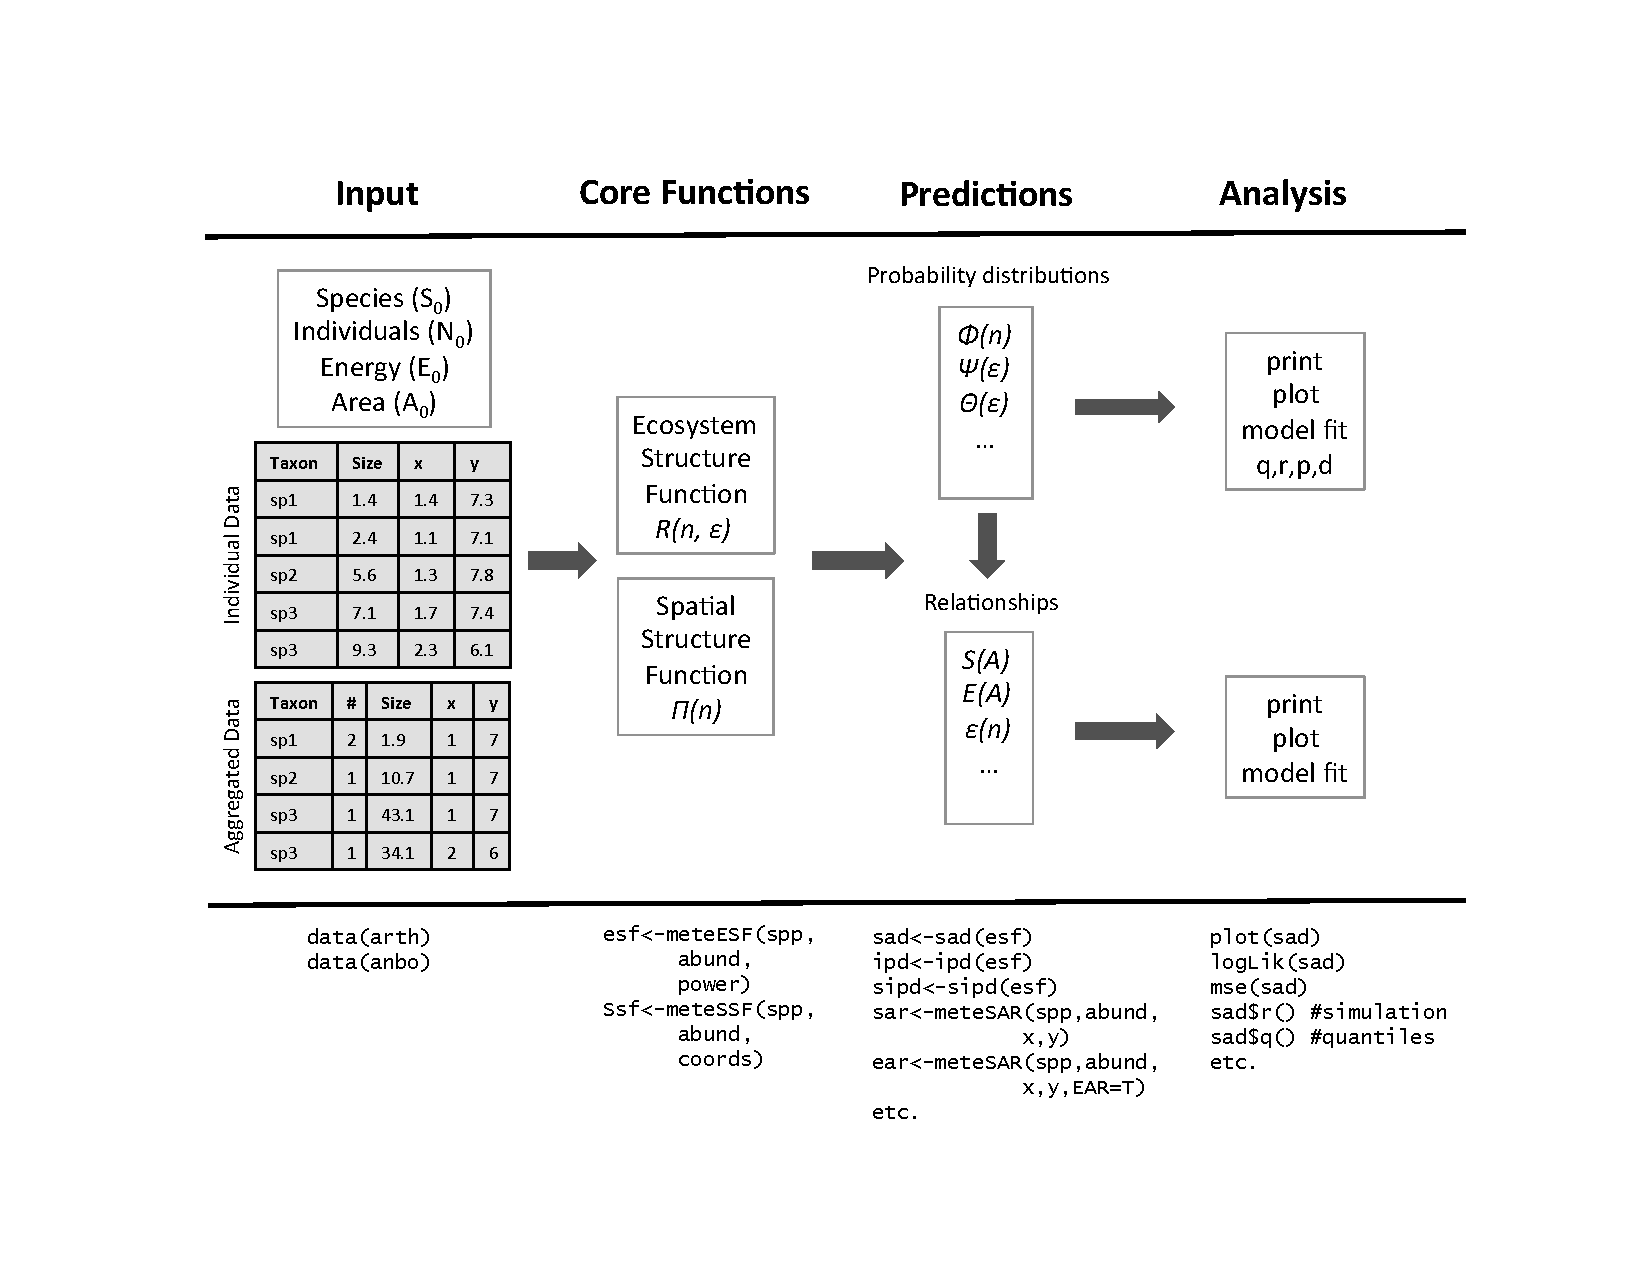
\includegraphics[width=\textwidth]{figs/meteR_workflow.pdf}
    \caption[\texttt{meteR}'s workflow]{\texttt{meteR}'s
      workflow. \texttt{meteR} accepts multiple data types, which are
      used to calculate the core probability distributions from which
      all predictions arise: the \textit{Ecosystem Structure Function}
      (ESF) and the \textit{Spatial Structure Function} (SSF). From
      the ESF and SSF, a variety of macroecological distributions can
      be calculated (see Table \ref{tab:metrics} for
      definitions). Each of these can be plotted or summarized in
      various ways and model fit is readily assessed. Furthermore,
      density, distribution function, quantile function and random
      generation is available for each function, allowing for custom
      plotting, simulation and model evaluation.}
\label{fig:workflow}
\end{center} 
\end{figure}


\begin{figure}[!h] 
  \begin{center}
    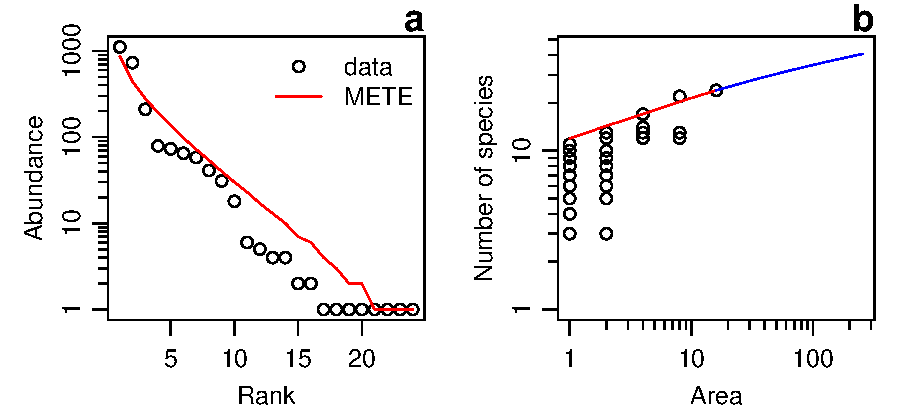
\includegraphics[width=0.75\textwidth]{figs/meteR_MS_v3-anbo_plot}
    \caption[Species abundance distribution and species area
    relationship for the \texttt{anbo} dataset]{Species abundance
      distribution (a) and species area relationship (b) for the
      \texttt{ anbo} dataset. The blue line in (b) depicts the
      upscaled SAR predicted by METE. METE fits the Anza Borrego data
      poorly at increasingly small scales. Understanding such
      systematic deviations from theory could be an opportune area of
      exploration, and initial work suggests that such deviations
      could be an indicator of anthropogenic disturbance (Newman
      \textit{et al.}, in prep.) such as invasive species, which are
      present in the Anza Borrego dataset. Note that we have stylized
      the log axes using custom code not included in \texttt{meteR}.}
\label{fig:anbo}
\end{center} 
\end{figure}


\begin{figure}[!h] 
  \begin{center}
    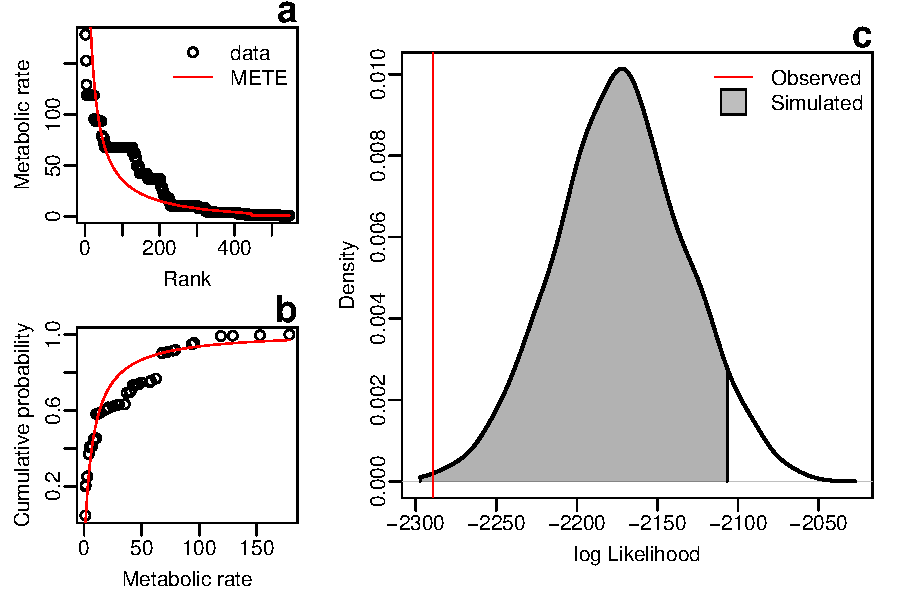
\includegraphics[width=0.75\textwidth]{figs/meteR_MS_v3-arth_plot}
    \caption[Individual power distributions shown]{Individual power
      distributions shown as a rank plot (a) and cumulative density
      plot (b). To evaluate model fit we compare the observed
      likelihood of the data given the METE model (red line in panel
      c) to simulated likelihoods produced by simulated \texttt{nrep}
      communities from the fitted METE object and calculating their
      likelihoods. Thus the simulated distribution represents
      hypothetical likelihoods for datasets obeying METE.}
\label{fig:arth} 
\end{center} 
\end{figure}

\section*{Tables}

%% for raggedright columns
\newcolumntype{L}[1]{>{\raggedright\let\newline\\\arraybackslash\hspace{0pt}}m{#1}}

\begin{table}[!h]
\caption[METE predictions]{METE predictions. Following notational
  conventions in \citet{Harte:2011ut}, $Z$ and $Z_{\Pi}$ are partition
  functions (i.e. to ensure their respective probability distributions
  to sum to 1), $\lambda_1$, $\lambda_2$, and $\lambda_\Pi$ are
  Lagrange multipliers, and commonly used combinations of them include
  $\beta = \lambda_1 + \lambda_2$, $\sigma = \lambda_1 +
  E_0\lambda_2$, and $\gamma=\lambda_{1} + \epsilon \lambda_{2}$.} 
\label{tab:metrics}
\small
\begin{tabular}{L{4cm} p{1.2cm} L{5.4cm} p{2cm} p{2cm}}
  \hline
 Predictions & Acronym & Functional Form & Type & \texttt{meteR} function\\ 
  \hline
      Ecosystem Structure Function & ESF & $R(n,\epsilon | N_0, S_0,E_0) = \frac{1}{Z} e^{-\lambda_1n} e^{-\lambda_2n\epsilon}$  & Core Distribution & \texttt{meteESF} \\ 
	Spatial Structure Function & SSF & $\Pi(n,|n_0, A, A_0) = \frac{1}{Z_\Pi} e^{-\lambda_\Pi n}$& Core Distribution & \texttt{meteSSF} \\
	Distribution of Species Abundance & SAD & $\Phi(n|N_0, S_0)\approx \frac{1}{log\frac{1}{\beta}} \frac{e^{\beta n}}{n}$ & Distribution & \texttt{sad} \\ 
 	Distribution of individual Power across community & IPD & $\Psi(\epsilon|N_0, S_0, E_0)\approx  \lambda_2 \cdot \beta \frac{e^{-\gamma}}{(1-e^{\gamma})^2} $& Distribution & \texttt{ipd} \\
	Distribution of individual Power for species with $n$ individuals & SIPD & $\Theta(\epsilon | n,N_0, S_0, E_0)\approx \lambda_2ne^{-\lambda_2n(\epsilon-1)}$ & Distribution & \texttt{sipd} \\
	Distribution of average (over individuals) metabolic rates over species & SPD & $\nu (\overline{\epsilon} |  N_0, S_0,E_0) \approx \frac{1}{log\frac{1}{\beta}}  \frac{e^{\beta / \lambda_2(\overline{\epsilon} -1)}}{\overline{\epsilon} -1}$ & Distribution & \texttt{spd} \\
	Average individual metabolic rate for species with $n$ individuals & ebar & $\overline{\epsilon}(n | N_0, S_0,E_0) \approx 1 + \frac{1}{n\lambda_2}$ & Relationship & \texttt{ebar} \\
	Species Area Relationship & SAR & $\bar{S}(A) = S_0 \sum_{n=1}^{N_0} \left(1 - \Pi(0 | n)\right) \Phi(n)$ & Relationship & \texttt{meteSAR}, \verb|downscaleSAR|, \verb|upscaleSAR| \\
	Endemics Area Relationship & EAR & $\bar{E}(A) = S_0 \sum_{n=1}^{N_0} \Pi(n | n) \Phi(n)$ & Relationship & \verb|meteSAR|, \verb|downscaleSAR| \\
   \hline
\end{tabular}
\end{table}


\renewcommand{\chaptername}{}
\chapter*{Conclusion}
\addcontentsline{toc}{chapter}{Conclusion}

Using two seminal paleontological datasets \citep{sepkoski1992,
  alroy08} I have shown that fluctuations in marine biodiversity over
the past 550 million years results from the superposition of many
independently fluctuating subsystems whose fluctuations are Gaussian
but give rise to non-Gaussian patterns when combined.  These
independent subsystems correspond to lineages of closely related
animal taxa, implying that diversification within lineages is driven
by random additive interactions with the environment. These findings
thus challenge the idea that changes in origination and extinction
through deep geologic time are the result of complicated evolutionary
interactions among organisms and between organisms and their
environment \citep{bak1993, sole1997, newman1995}. However, I
demonstrated that the evolutionary process responsible for generating
new lineages varies slowly through time, possibly driven by non-random
evolutionary innovations in the physiology and demography of new
lineages. This slow change between lineages produces patterns of
apparent complexity earlier ascribed to unnecessarily complicated
mechanisms. I have further shown, using permutational null models,
that these findings are not an artifact of how fossils are
taxonomically classified but rather capture true underlying biological
processes.

To further explore the importance of biological evolution in driving
unique non-equilibrial patterns I synthesized population genetic and
trophic network data for Hawaiian arthropods to show that as assembly
by immigration (in communities assembled on young substrates) gives
way to evolutionary processes (in communities assembled on old
substrates), arthropod herbivore networks momentarily reach a steady
state as predicted by equilibrial statistical mechanics
\citep{rominger2015GEB}. On the young and old end of this spectrum
different eco-evolutionary mechanisms lead to deviations from
statistical mechanical theory: incomplete assembly and non-equilibrium
adaptive evolution, respectively. Using population genetic data from
other arthropod lineages I show that assembly and differentiation
rates differ according to the trophic level of the organisms, implying
that different trophic levels will reach an equilibrium at different
periods and for different durations along the chronosequence.  This
study provides a framework for using island systems combined with
simple equilibrial theory building to understand how complex
communities emerge from ecological (population dynamics, dispersal,
trophic interactions) and evolutionary (genetic structuring,
adaptation, speciation, extinction) processes.

Finally, I argue that to fully realize the utility of statistical
mechanics in the study of biodiversity, we must test these theories
across many different systems.  I advocate for further exploring how
the evolutionary process and rapid ecological transitions could drive
deviations from theory by proposing tests of the maximum entropy
theory of ecology \citep{harte2011} across gradients of disturbance,
diversity and evolutionary age.  To facilitate these novel tests I
provided ecologists with the open source \texttt{R} package
\texttt{meteR}.

``Top-down'' approaches to biodiversity theory will be critical for
building universal predictions about the the diversity of life
\citep{harte2011, krakauer2011}.  These theories require that many
biological details be course-grained but in turn promise unprecedented
predictive power.  Testing these theories in real ecosystems can
illuminate where more detailed, biologically-grounded mechanisms are
further needed.  In this thesis I have used principles form
statistical mechanics to develop and test new top-down theory that
explains fluctuations in diversity through deep geologic time and
identifies key evolutionary processes as important mechanisms to
include in a synthetic eco-evolutionary theory of biodiversity.  This
work motivates exciting research directions for the near future which
I sketch below.

% how has thesis provided better top-down predictive theory for
% biodiversity and better integrated evolution into theory?

% use of stat mech to make detailed top-down predictions and to
% identify where other mechanisms needed

% application of top down modeling to evolutionary process and testing
% of top down theory in evolving landscapes to understand how
% evolutionary drives deviation from theory

% provided software tools to make theory testing more robust and
% accessible

% what future steps are motivated by the thesis?

\section{Future Work}

\subsection{Adaptive landscapes and non-Markovian memory}

Ecological theory has of late been dominated by neutral models
\citep[e.g.][]{rominger2009, rominger2015GEB}. This approach needs
robust alternative hypotheses because a lack of alternative theories
rooted in classical ecology could be one limitation preventing a more
rigorous competition between deterministic and statistical theories of
biodiversity. My work with super-statistics in the fossil record
(Chapter 1) motivates a new approach to ecological theory using
super-statistics to parsimoniously capture the non-neutrality of
species and relate that non-neutrality to the non-equilibrium process
of diversification on an adaptive landscape.

\subsection{Metabarcoding and Ecological Theory}

Combining test of ecological theory with massive phylogenetic data, as
motivated by my synthesis of population genetics with trophic networks
(Chapter 2), could determine what aspects of evolutionary history
specifically shape ecological communities, but massive phylogenetic
data on the scale of large ecological studies is limiting.  A new
approach dubbed ``metabarcoding'' \citep{taberlet2012} harnesses next
generation sequencing technology to produce massive amounts of genetic
data for ecological samples. This approach, however, has known
pitfalls \citep[e.g. bias in primer affinities between
taxa][]{clarke2014} but these could be overcome bioinformatically
using hierarchical models, already commonplace in ecology
\citep{royleDorazio}.

\printbibliography[heading=subbibliography]

\appendix
\chapter{Supplement to ``Punctuated non-equilibrium and niche conservatism explain
  biodiversity fluctuations through the Phanerozoic''}

\section{Limit distribution of a time-averaged homogeneous
  origination-extinction process}
\label{sec:suppLimitDist}
Fossil taxa gain and lose taxa according to an origination-extinction
process. We assume that most fossil occurrences of a taxon come from
the period of its history when it is dominant and in steady state. In
a time slice of duration $\tau$ during such a period of steady state
the latent per capita rates of origination and extinction would be
equal (i.e. $\lambda = \mu \equiv \rho$) and the number of origination
or extinctions events (call such events $Y$) each follow an
inhomogeneous Poisson process with rate $\rho N_t$ where $N_t$ is the
number of species or genera in the taxon of interest at time
$t$. Allowing $N_t$ to vary smoothly with time, and invoking the
comunicative property of the Poisson distribution, we arrive at the
number $Y$ of extinction \emph{or} origination events in $\tau$ being
distributed
\begin{equation}
  \label{eq:eventPois1}
  Y \sim \text{Pois}(\rho \int_{t=0}^\tau N(t) dt).
\end{equation}
Under the steady state assumption we can approximate $N(t)$ by
$\bar{N}$, the steady state diversity, leading to
\begin{equation}
  \label{eq:eventPois2}
  Y \sim \text{Pois}(\rho \bar{N} \tau).
\end{equation}

Assuming the $\tau$ of each time period in the Paleobiology Database
or Sepkoski's compendium to be approximately equal (i.e. equal
durations of major stratographic units) then the distribution of
fluctuations within taxa will be asymptotically Gaussian.

\section{Additional super-statistical analyses}
To evaluate the sensitivity of our super-statistical analysis on the
particular data used and we tested our predictions on different data
sets (see below). The fact that it works in all different applications
indicates that it is robust to vagaries of different recording
strategies and bias corrections in paleobiology. This could mean that
much of the raw signal in massive fossil datasets, at least signals
regarding fluctuations, are not artifacts of sampling, as has been
proposed before \cite{hannisdal2011}.

\subsection{Raw PBDB data} \label{sec:rawPBDB}
We calculated the super-statistical prediction at the order level from
raw genus diversity recorded in the PBDB without correcting for
taphonomic or sampling bias (Fig. \ref{fig:supp_rawPBDB_Px}). The
super-statistical calculation also closely fits the raw data as in the
case of sampling and publication bias-corrected data.

\subsection{Different taxonomic ranks in PBDB data}
As noted in the main text, the super-statistical prediction
predictably breaks down at higher taxonomic scales. In Figure
\ref{fig:supp_PBDB_Px_cls} we present this worsening fit graphically
using class level data with three-timer and publication corrected PBDB
data

\subsection{Sepkoski's compendium} \label{sec:suppSepk}
Sepkoski's compendium \cite{sepkoski1992} provided the first
hypothesis of Phanerozoic diversification.  As such, it has served as
a benchmark for further investigation into large-scale paleobiological
patterns\cite{alroy08}.  We conducted the same super-statistical
analysis as in the main text and find comparable results.
Specifically, the super-statistical prediction far out preforms the
null Gaussian model (Fig. \ref{fig:supp_sepkPx}) and worsens with
increasing taxonomic scale (Fig. \ref{fig:supp_sepkPx}), again
implying the uniqueness of orders.

% \clearpage

% \bibliographystyle{pnas}
% \bibliography{../../bib/superStat}

\clearpage

\section*{Supplemental Figures}

\begin{figure}[!hp]
  \centering
%  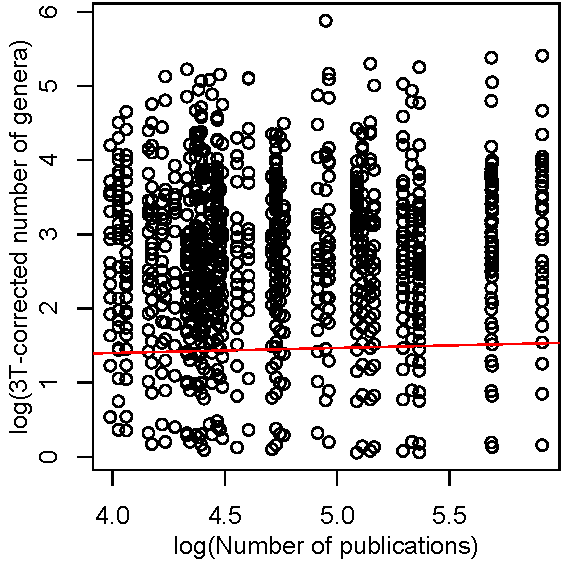
\includegraphics[scale=0.7]{figSupp_divByPub.pdf}
  \caption[Relationship between number of publications and genus
  diversity]{Relationship between number of publications and genus
    diversity as recorded by the PBDB.}
  \label{fig:divByPub}
\end{figure}

\begin{figure}[!hp]
  \centering
%  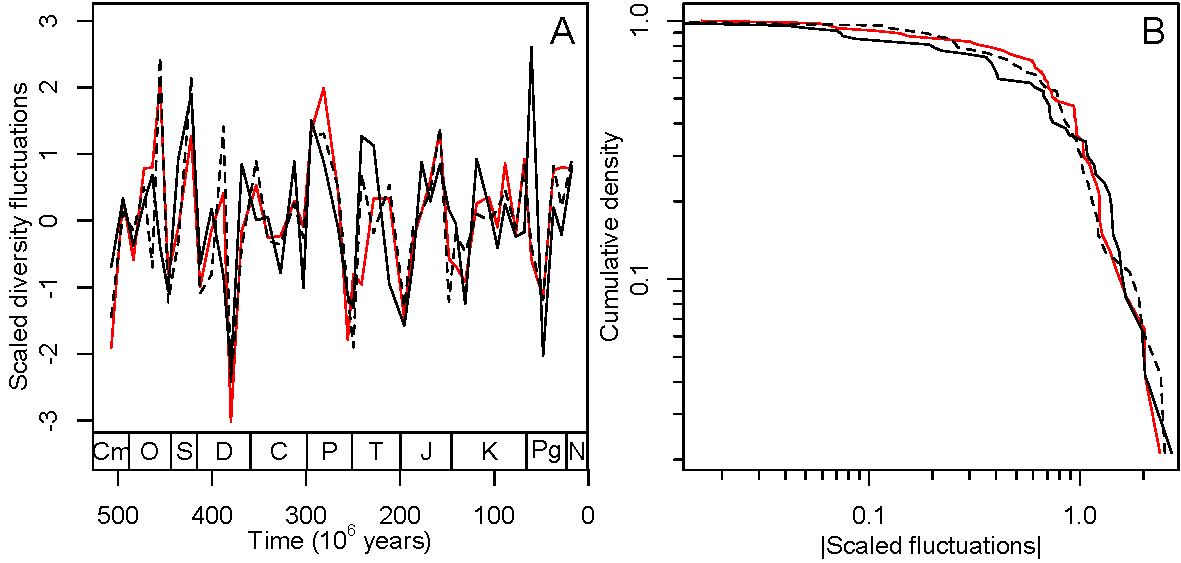
\includegraphics[scale=0.7]{figSupp_sqsRaw3tpub.pdf}
  \caption[Comparison of SQS method with the raw data and three-timer
  bias correction method]{Comparison of SQS method \cite{alroy2010}
    (solid black line) with the raw data (dashed black) and our
    three-timer and publication bias correction method (red). The
    time-series of all marine invertebrate genera shows general
    agreement with the only major deviations toward the modern
    (A). Despite these differences the distribution of fluctuations in
    genus diversity across all marine invertebrates show good
    agreement (B).}
  \label{fig:supp_3TPub}
\end{figure}

\begin{figure}[!hp]
  \centering
%  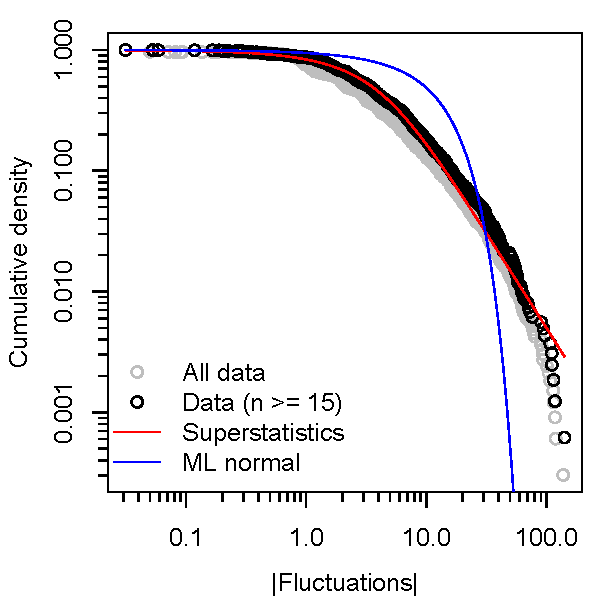
\includegraphics[scale=0.7]{figSupp_pbdbRaw_Px.pdf}
  \caption[Super-statistical prediction of raw data]{Super-statistical
    prediction of raw (i.e. not bias corrected) order-level
    fluctuations in genus diversity recorded in the PBDB. Grey dots
    are the full data of orders, while black ones are orders with more
    than 15 points. The red line is our theoretical prediction and the
    blue line the best Gaussian fit to the data.}
  \label{fig:supp_rawPBDB_Px}
\end{figure}

\begin{figure}[!hp]
  \centering
%  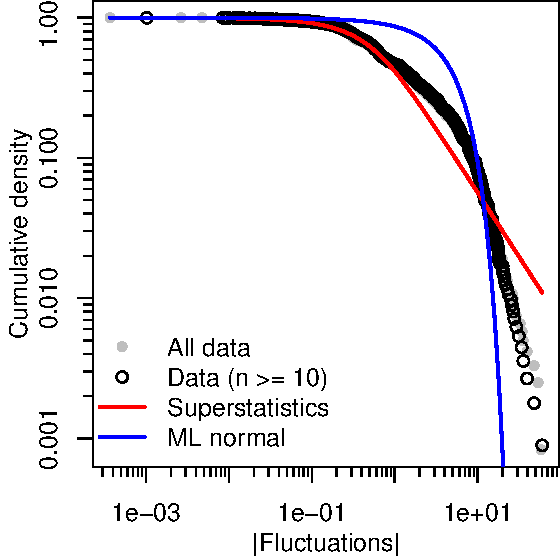
\includegraphics[scale=0.7]{figSupp_Px_cls.pdf}
  \caption[Super-statistical prediction of bias corrected class-level
  data]{Super-statistical prediction of bias corrected class-level
    fluctuations in genus diversity recorded in the PBDB. Grey dots
    are the full data of orders, while black ones are orders with more
    than 15 points. The red line is our theoretical prediction and the
    blue line the best Gaussian fit to the data. Note at the class
    level the fit is predictably worse, see main text for discussion.}
  \label{fig:supp_PBDB_Px_cls}
\end{figure}

\begin{figure}[!hp]
  \centering
%  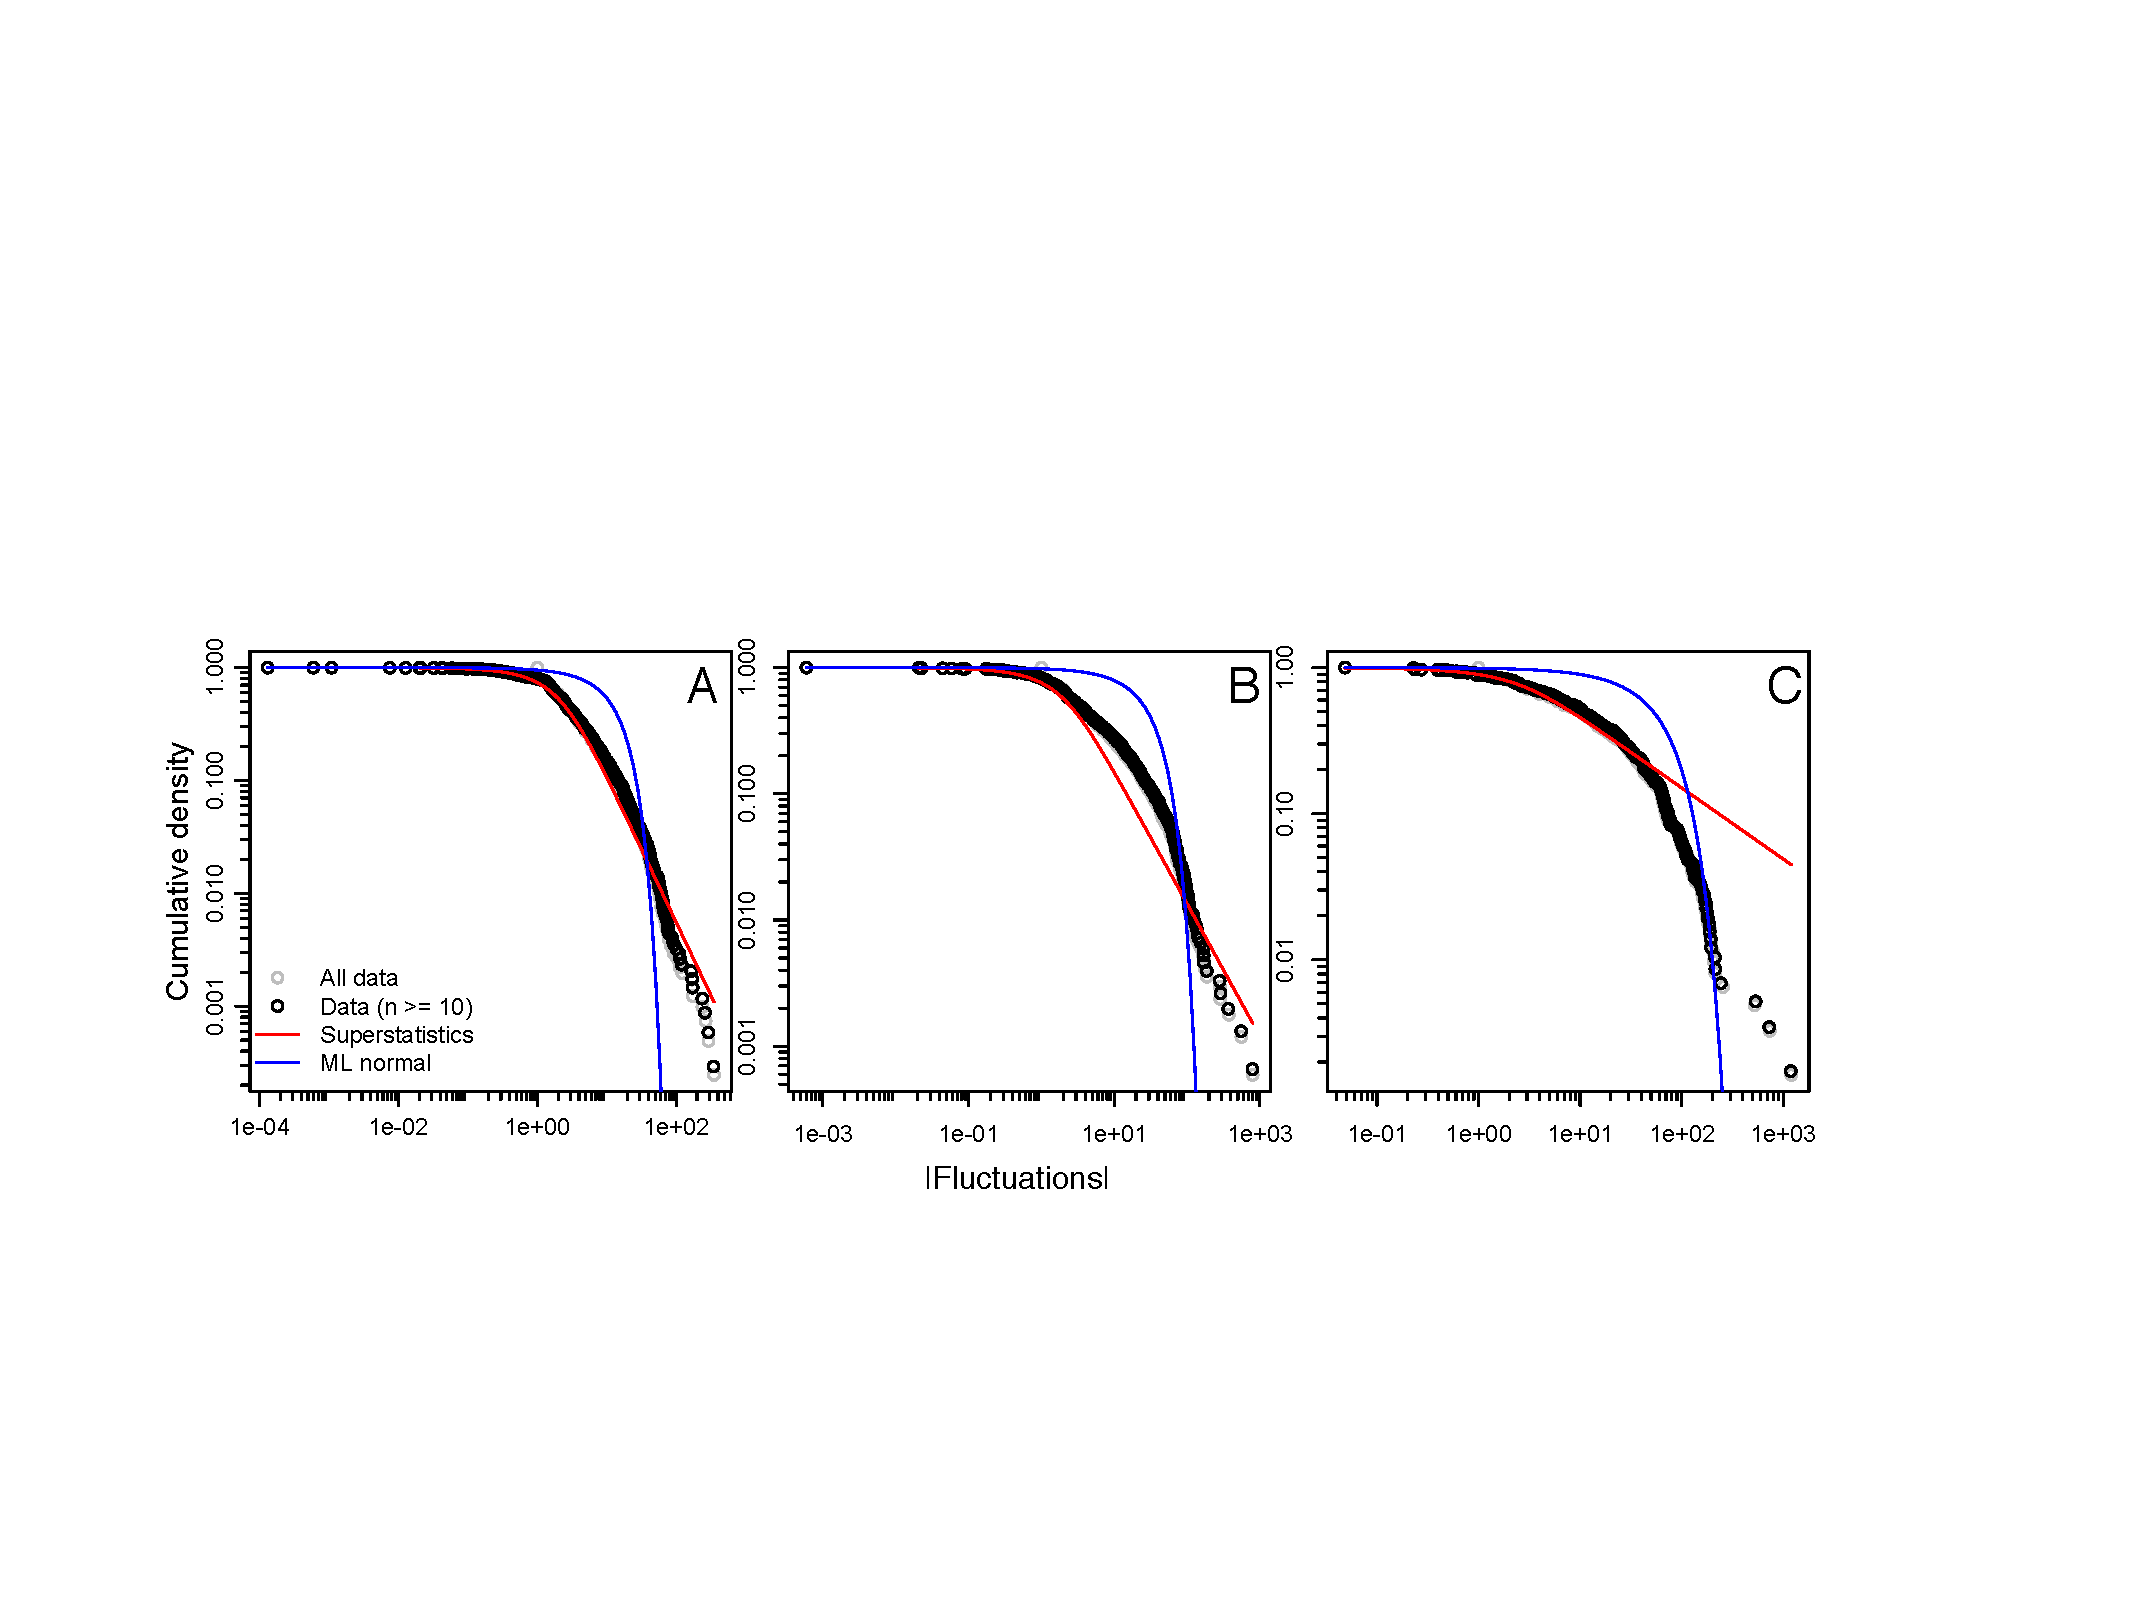
\includegraphics[scale=0.6]{figSupp_sepk_Px.pdf}
  \caption[Super-statistical prediction for Sepkoski's
  compendium]{Super-statistical prediction (red line) of fluctuations
    in genus diversity recorded in Sepkoski's compendium of marine
    invertebrates compared to maximum likelihood normal distribution
    (blue line). Super-statistical theory explains order level
    fluctuations well (A) with increasingly poorer fits at the class
    (B) and phylum (C) levels.}
  \label{fig:supp_sepkPx}
\end{figure}


\chapter{Supplement to ``Community assembly on isolated islands:
  Macroecology meets evolution''}
\label{supp:ch2}

\section{Compilation of networks and metric validation}

Researchers have put forward a set of ``network metrics,'' including
nestedness \citep{bascompte2003, ulrich2009} and modularity
\citep{newman2004, olesen2007}, to understand the complex structure of
ecological networks. Null models are used to evaluate the statistical
significance of these metrics and to compare between networks of
different size \citep{ulrich2009}. We compare the results derived from
two common null models: the ``probabilistic null'' of
\cite{bascompte2003} using the relative degree distributions of plants
and herbivores as weights while randomizing links and suffers from
high Type II error \citep{ulrich2009}; the ``fixed-fixed null''
\citep{ulrich2009} maintains the exact number of links assigned to
each species while randomizing which interactors fill the requisite set
of links and suffers from high Type I error \citep{ulrich2009}. We find that
using these different null models does not change any trends in our
network statistics across the Hawaiian chronosequence but different
null models do influence the sign and significance of the network
metrics (Fig. \ref{figSupp:netMetComp}). We therefore do not interpret
the sing or significance of the metrics but only their relative trends
across site age.

Because these networks are based on opportunistic data associated with
species descriptions, and not based on standardized ecological
surveys, we cannot interpret patterns in network metrics without
evaluating possible sampling biases \citep{nielsen2007, gibson2011,
  rivera2012}.  To do so we rarify networks by the number of Hemiptera
species included and, for each subsampled network, re-calculate
nestedness and modularity z-scores. This rarefaction procedure shows
that nestedness is very sensitive to network size
(Fig. \ref{figSupp:rfy}), a known property of nestedness
\citep{nielsen2007, gibson2011, rivera2012}. However the relative
nestedness z-scores across networks remain qualitatively similar to
those observed for the complete networks (Fig. \ref{figSupp:rfy}).
Modularity depends on network size in a more variable way
(Fig. \ref{figSupp:rfy}). Modularity is expected to decrease with
network size \citep{rivera2012} and so the marked increase in
modularity with network size on Haleakala is unexpected. However in
light of the large number of highly specialized taxa this pattern is
more reasonable---if most species only have within module links then
removing these species through subsampling will only reduce overall
modularity.  Thus this pattern speaks to the high level of
specialization on Haleakala, and to a lesser extent at Kokee which
also shows a slight increase in modularity with network size
(Fig. \ref{figSupp:rfy}).


\section{\texttt{R} Scripts for Maximum Entorpy Analysis and Monte
  Carlo Methods}
\label{sec:meteCode}

\subsection{Needed Functions}

\begin{verbatim}
require(distr)

## d, p and r functions for the maxent link distribution
## also a funciton to calculate the MLE and log likelihood

dmelink <- function(x, la) {
    exp(-la*(x-1)) - exp(-la*x)
}

pmelink <- function(x, la, lower.tail=TRUE) {
    if(length(x) > 1) {
        cp <- sapply(x, function(q) sum(dmelink(1:q, la)))
    } else {
        cp <- sum(dmelink(1:x, la))
    }
    
    if(lower.tail) {
        return(cp)
    } else {
        return(1 - cp)
    }
}

rmelink <- function(n, la, X0) {
    sample(X0, n, rep=TRUE, prob=dmelink(1:X0, la))
}


qmelink <- function(x, la) {
    fun <- DiscreteDistribution(1:3000, dmelink(1:3000, la))
    fun@q(x)
}

## likelihood functions (for simple cases maxent solution is equivilant 
## to maximum likelihood solution so we use MLE for computational ease)
melink.mle <- function(x) {
    log(1 + 1 / mean(x - 1))
}

melink.logLik <- function(x) {
    la <- melink.mle(x)
    
    length(x) * log(1 - exp(-la)) - la * sum(x - 1)
}


## function to make rank function (for plotting) of maxent link distrib
melink.rankFun <- function(x) {
    qmelink(seq(1-1/(length(x)+1), 1/(length(x)+1), 
                by=-1/(length(x)+1)), melink.mle(x))
}

## mean squared error function for maxent link distrib
melink.mse <- function(x) {
    mean((sort(x, TRUE) - melink.rankFun(x))^2)
}

## monte carlo method for calculating distribution of mse values 
## under model where maxent truely generated the link distribution
sim.melink.z <- function(x, X0, nsim=999) {
    la <- melink.mle(x)
    
    res <- replicate(nsim, {
        # browser()
        sim <- rmelink(length(x), la, X0)
        return(melink.mse(sim))
    })
    
    obs.mse <- melink.mse(x)
    
    return(list(obs=obs.mse, z=(obs.mse - mean(res)) / sd(res), sim=res))
}
\end{verbatim}

\subsection{Example Use}

\begin{verbatim}
## set a Lagrange multiplier value and simulate data
la <- 0.01

## fit the maxEnt model to simulated data
x <- rmelink(2000, la, 2000)

## evalute if fitted maxEnt model matches the data
melink.mle(x) # the MLE should be near 0.01
plot(sort(x, TRUE)) # the plotted data should look like the theory
lines(pmelink(1:200, melink.mle(x)), col='red')

## test that the logLike function is returning the correct value
melink.logLik(x) - sum(log(dmelink(x, melink.mle(x)))) < 1e-12

## test that the log likelihood simulation is working
sim.melink.z(x, 200) # should be a small z-value
sim.melink.z(rbinom(100, 200, 0.1), 200) # should be a large z-value
\end{verbatim}

\printbibliography

\clearpage

\section*{Supplemental Figures}

\begin{figure}[!hp]
  \centering
  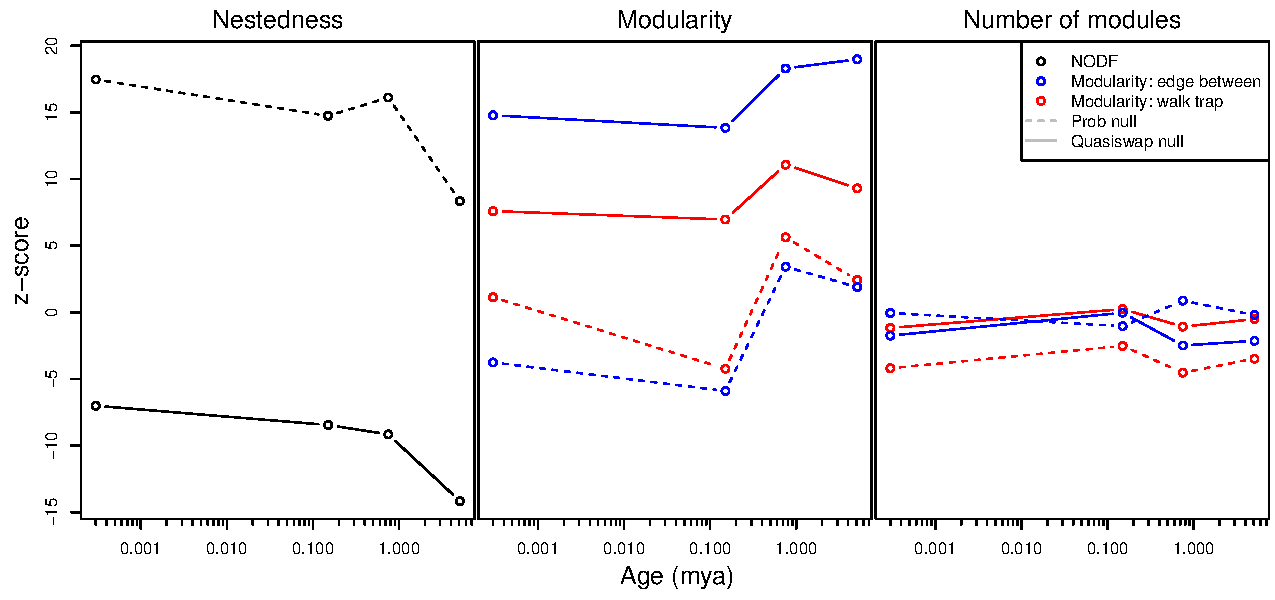
\includegraphics[scale=0.6]{figs/figSupp_netMetComp.pdf}
  \caption[Comparison of different null models]{Comparison of
    different null models (``Prob'' and ``Quasiswap'') used to
    standardize network metrics and comparison of different algorithms
    for assessing modularity (``edge between'' and ``walk
    drap''). Choice of null model has a strong influence on the sign
    and magnitude of metrics but not on their relative trends. The
    different modularity algorithms lead to largely similar
    qualitative patterns.}
  \label{figSupp:netMetComp}
\end{figure}

\begin{figure}[!hp]
  \centering
  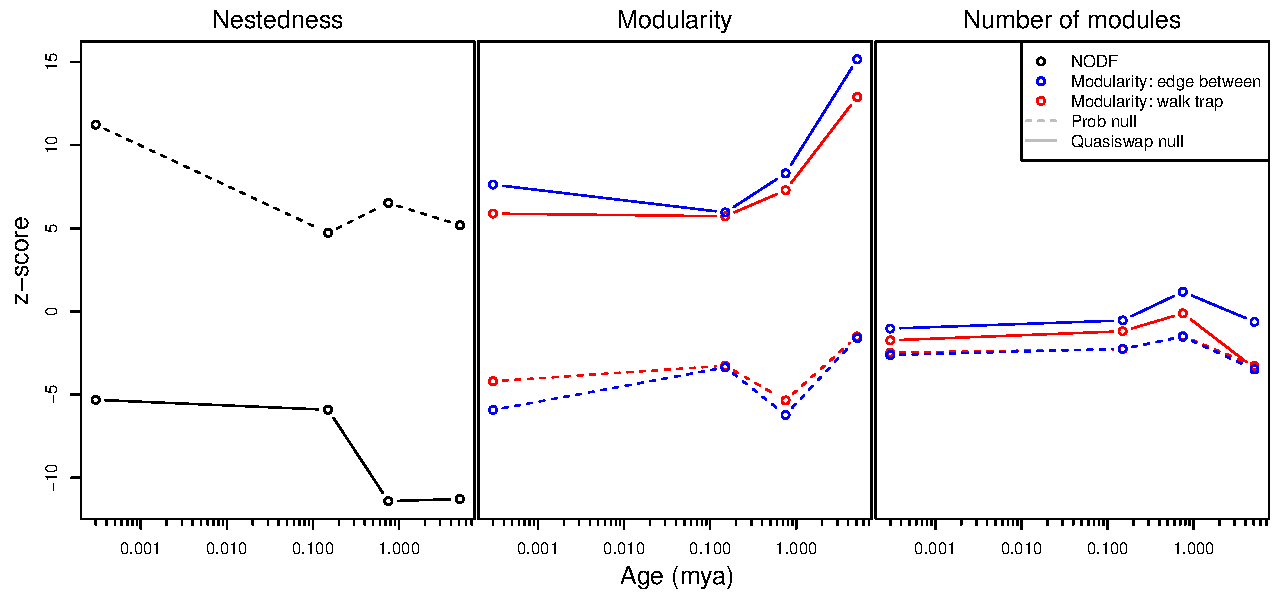
\includegraphics[scale=0.6]{figs/figSupp_netMetCons.pdf}
  \caption[NODF and modularity for non-conservative networks]{Metrics
    NODF and modularity calculated for networks based on more
    biogeographically conservative assignment of Hemiptera to
    localities. Colors and metric specifics as in Figure
    \ref{figSupp:netMetComp}.}
  \label{figSupp:netCons}
\end{figure}

\begin{figure}[!hp]
  \centering
  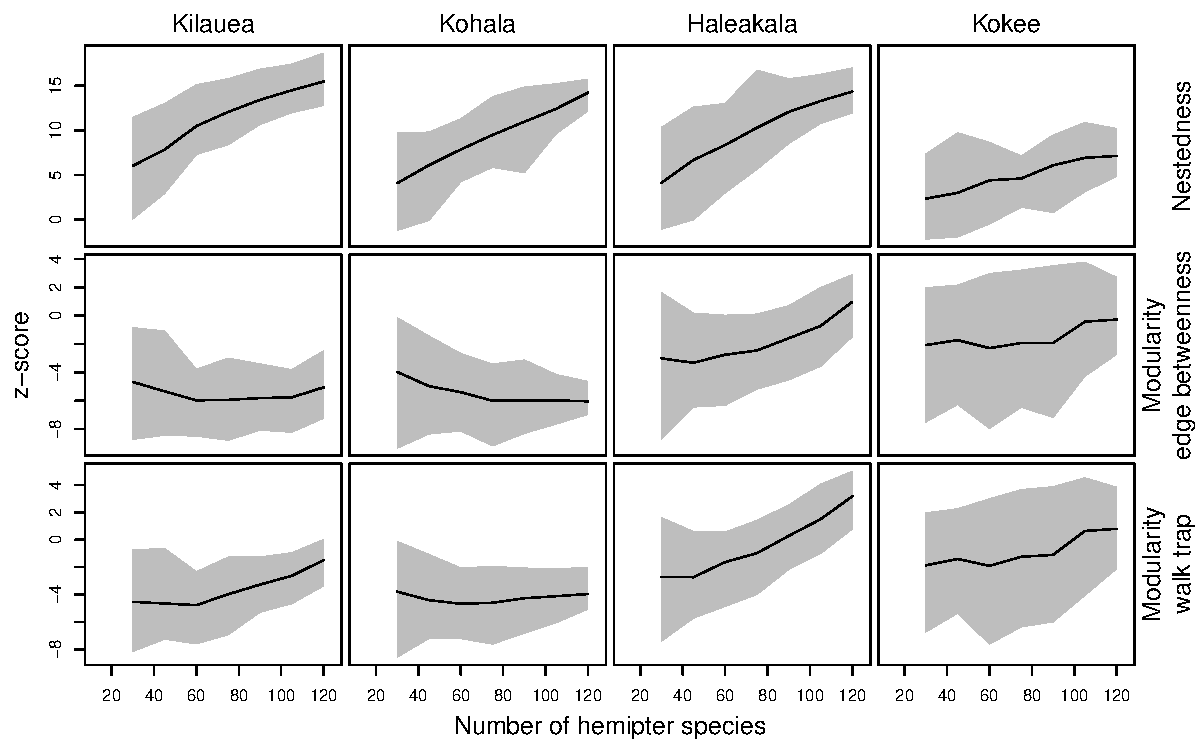
\includegraphics[scale=0.6]{figs/figSupp_rarified_prob1.pdf}
  \caption[Result from rarification analysis]{Result from rarification
    analysis showing sensitivity of network metrics to number of
    Hemiptera sampled.}
  \label{figSupp:rfy}
\end{figure}



\bibliographystyle{thesis}
\bibliography{thesis}

\end{document}
